% ============================================================================
% English version: the same sections as article.tex in a generic single-column
% layout for a Scopus-indexed venue chosen later. Switching venues = replacing the
% preamble and \bibliographystyle (sections, tables and figures stay): e.g. llncs +
% splncs04 (Springer CCIS/LNCS),
% elsarticle + elsarticle-num (Elsevier), or the journal's own class.
% Tables: tables/*_en.tex (booktabs, decimal point); numbers: tables/numbers_en.tex;
% figures: ../figures/en/; references: references.bib (DOI fields kept for the venue style).
% Before submission: \draftnotesfalse hides every \todo.
% ============================================================================
\documentclass[11pt, a4paper]{article}

\usepackage[utf8]{inputenc}
\usepackage[T1]{fontenc}
\usepackage[english]{babel}

\usepackage[left=28mm, right=28mm, top=25mm, bottom=28mm]{geometry}
\usepackage{amsmath, amssymb}
\usepackage{graphicx}
\graphicspath{{../figures/en/}}
\usepackage{float}
\usepackage{booktabs}
\usepackage{xcolor}
\usepackage{enumitem}
\usepackage{caption}
\captionsetup{labelfont=bf, labelsep=period}
\emergencystretch=1.5em

\usepackage[hidelinks]{hyperref}

% АВТОГЕНЕРАЦИЯ / AUTOGENERATED: build_tables.py <- metrics/*.csv
% Макросы с ключевыми числами для прозы; значения уже отформатированы для языка версии.
% Пример: overlap@10 стратегии bal при опросе одного шарда — \balOverlapAtOne, её ДИ — \balOverlapAtOneCI,
% прирост над hash_bal — \balGainOne \balGainOneCI, на OOD — \balOodGainOne.
\newcommand{\nDocs}{241,185}
\newcommand{\nJudgedDocs}{128,009}
\newcommand{\nDistractors}{113,176}
\newcommand{\nQueries}{122,063}
\newcommand{\nTrainQueries}{115,959}
\newcommand{\nHoldoutQueries}{6,104}
\newcommand{\nVocabulary}{189,841}
\newcommand{\nDocTermPairs}{6,320,007}
\newcommand{\termsPerDoc}{26.2}
\newcommand{\maxDfShare}{11.4}
\newcommand{\nTermsOverOnePct}{383}
\newcommand{\nTermsOverFivePct}{11}
\newcommand{\nGraphTerms}{10,567}
\newcommand{\nGraphEdges}{39,794}
\newcommand{\nGraphComponents}{289}
\newcommand{\nLargestComponent}{9,972}
\newcommand{\graphVocabularyShare}{5.6}
\newcommand{\nFrameWords}{29}
\newcommand{\nTrain}{9,980}
\newcommand{\nHoldout}{6,093}
\newcommand{\nOod}{10,000}
\newcommand{\nConnectedPairs}{2,000}
\newcommand{\nConnectedTriples}{2,000}
\newcommand{\nFrequentPairs}{2,000}
\newcommand{\nFrequentTriples}{2,000}
\newcommand{\leidenClusters}{340}
\newcommand{\leidenLargestCluster}{1,563}
\newcommand{\leidenModularity}{0.601}
\newcommand{\leidenFocusShards}{132}
\newcommand{\leidenFocusOverlapAtOne}{0.780}
\newcommand{\leidenFocusOodOverlapAtOne}{0.664}
\newcommand{\leidenFocusGainOne}{+0.083}
\newcommand{\leidenFocusGainOneCI}{[0.077,\,0.089]}
\newcommand{\cpmClusters}{2,211}
\newcommand{\cpmLargestCluster}{53}
\newcommand{\cpmModularity}{0.413}
\newcommand{\cpmFocusShards}{136}
\newcommand{\cpmFocusOverlapAtOne}{0.758}
\newcommand{\cpmFocusOodOverlapAtOne}{0.651}
\newcommand{\cpmFocusGainOne}{+0.061}
\newcommand{\cpmFocusGainOneCI}{[0.056,\,0.067]}
\newcommand{\infomapClusters}{1,119}
\newcommand{\infomapLargestCluster}{395}
\newcommand{\infomapModularity}{0.467}
\newcommand{\infomapFocusShards}{134}
\newcommand{\infomapFocusOverlapAtOne}{0.770}
\newcommand{\infomapFocusOodOverlapAtOne}{0.659}
\newcommand{\infomapFocusGainOne}{+0.072}
\newcommand{\infomapFocusGainOneCI}{[0.066,\,0.078]}
\newcommand{\metisClusters}{335}
\newcommand{\metisLargestCluster}{58}
\newcommand{\metisModularity}{0.144}
\newcommand{\metisFocusShards}{140}
\newcommand{\metisFocusOverlapAtOne}{0.743}
\newcommand{\metisFocusOodOverlapAtOne}{0.609}
\newcommand{\metisFocusGainOne}{+0.045}
\newcommand{\metisFocusGainOneCI}{[0.040,\,0.050]}
\newcommand{\hashBaseShards}{680}
\newcommand{\hashBaseDuplication}{25.7}
\newcommand{\hashBaseLargest}{15.7}
\newcommand{\hashBaseFanout}{3.23}
\newcommand{\hashBaseFanoutCI}{[3.19,\,3.26]}
\newcommand{\hashBaseSingleShard}{6.6}
\newcommand{\hashBaseTopShardTraffic}{0.3}
\newcommand{\hashBaseOverlapAtOne}{0.651}
\newcommand{\hashBaseOverlapAtOneCI}{[0.643,\,0.659]}
\newcommand{\hashBaseVolumeAtOne}{3.9}
\newcommand{\hashBaseOverlapAtTwo}{0.954}
\newcommand{\hashBaseOverlapAtTwoCI}{[0.951,\,0.958]}
\newcommand{\hashBaseVolumeAtTwo}{8.0}
\newcommand{\hashBaseOverlapAtThree}{0.996}
\newcommand{\hashBaseOverlapAtThreeCI}{[0.995,\,0.997]}
\newcommand{\hashBaseVolumeAtThree}{11.7}
\newcommand{\hashBaseOverlapAtFive}{1.000}
\newcommand{\hashBaseOverlapAtFiveCI}{[0.999,\,1.000]}
\newcommand{\hashBaseVolumeAtFive}{14.8}
\newcommand{\hashBaseOverlapAtFull}{1.000}
\newcommand{\hashBaseOverlapAtFullCI}{[1.000,\,1.000]}
\newcommand{\hashBaseVolumeAtFull}{15.2}
\newcommand{\hashBaseOodOverlapAtOne}{0.477}
\newcommand{\hashBaseOodFanout}{4.62}
\newcommand{\baseShards}{680}
\newcommand{\baseDuplication}{16.6}
\newcommand{\baseLargest}{79.4}
\newcommand{\baseFanout}{2.61}
\newcommand{\baseFanoutCI}{[2.58,\,2.64]}
\newcommand{\baseSingleShard}{13.8}
\newcommand{\baseTopShardTraffic}{9.8}
\newcommand{\baseMixedQueries}{55.3}
\newcommand{\baseOverlapAtOne}{0.796}
\newcommand{\baseOverlapAtOneCI}{[0.789,\,0.803]}
\newcommand{\baseVolumeAtOne}{35.0}
\newcommand{\baseOverlapAtTwo}{0.982}
\newcommand{\baseOverlapAtTwoCI}{[0.980,\,0.985]}
\newcommand{\baseVolumeAtTwo}{67.4}
\newcommand{\baseOverlapAtThree}{0.999}
\newcommand{\baseOverlapAtThreeCI}{[0.999,\,1.000]}
\newcommand{\baseVolumeAtThree}{85.6}
\newcommand{\baseOverlapAtFive}{1.000}
\newcommand{\baseOverlapAtFiveCI}{[1.000,\,1.000]}
\newcommand{\baseVolumeAtFive}{93.5}
\newcommand{\baseOverlapAtFull}{1.000}
\newcommand{\baseOverlapAtFullCI}{[1.000,\,1.000]}
\newcommand{\baseVolumeAtFull}{94.1}
\newcommand{\baseOodOverlapAtOne}{0.729}
\newcommand{\baseOodFanout}{3.83}
\newcommand{\baseRtwoShards}{680}
\newcommand{\baseRtwoDuplication}{19.3}
\newcommand{\baseRtwoLargest}{95.9}
\newcommand{\baseRtwoFanout}{2.31}
\newcommand{\baseRtwoFanoutCI}{[2.29,\,2.33]}
\newcommand{\baseRtwoSingleShard}{19.6}
\newcommand{\baseRtwoTopShardTraffic}{13.5}
\newcommand{\baseRtwoMixedQueries}{55.3}
\newcommand{\baseRtwoOverlapAtOne}{0.839}
\newcommand{\baseRtwoOverlapAtOneCI}{[0.833,\,0.847]}
\newcommand{\baseRtwoVolumeAtOne}{52.1}
\newcommand{\baseRtwoOverlapAtTwo}{0.989}
\newcommand{\baseRtwoOverlapAtTwoCI}{[0.987,\,0.991]}
\newcommand{\baseRtwoVolumeAtTwo}{89.2}
\newcommand{\baseRtwoOverlapAtThree}{1.000}
\newcommand{\baseRtwoOverlapAtThreeCI}{[1.000,\,1.000]}
\newcommand{\baseRtwoVolumeAtThree}{105.5}
\newcommand{\baseRtwoOverlapAtFive}{1.000}
\newcommand{\baseRtwoOverlapAtFiveCI}{[1.000,\,1.000]}
\newcommand{\baseRtwoVolumeAtFive}{110.0}
\newcommand{\baseRtwoOverlapAtFull}{1.000}
\newcommand{\baseRtwoOverlapAtFullCI}{[1.000,\,1.000]}
\newcommand{\baseRtwoVolumeAtFull}{110.3}
\newcommand{\baseRtwoOodOverlapAtOne}{0.833}
\newcommand{\baseRtwoOodFanout}{3.33}
\newcommand{\baseRthreeShards}{680}
\newcommand{\baseRthreeDuplication}{21.1}
\newcommand{\baseRthreeLargest}{98.4}
\newcommand{\baseRthreeFanout}{2.18}
\newcommand{\baseRthreeFanoutCI}{[2.16,\,2.21]}
\newcommand{\baseRthreeSingleShard}{23.2}
\newcommand{\baseRthreeTopShardTraffic}{15.0}
\newcommand{\baseRthreeMixedQueries}{55.3}
\newcommand{\baseRthreeOverlapAtOne}{0.852}
\newcommand{\baseRthreeOverlapAtOneCI}{[0.845,\,0.858]}
\newcommand{\baseRthreeVolumeAtOne}{58.4}
\newcommand{\baseRthreeOverlapAtTwo}{0.990}
\newcommand{\baseRthreeOverlapAtTwoCI}{[0.989,\,0.992]}
\newcommand{\baseRthreeVolumeAtTwo}{92.6}
\newcommand{\baseRthreeOverlapAtThree}{1.000}
\newcommand{\baseRthreeOverlapAtThreeCI}{[1.000,\,1.000]}
\newcommand{\baseRthreeVolumeAtThree}{105.5}
\newcommand{\baseRthreeOverlapAtFive}{1.000}
\newcommand{\baseRthreeOverlapAtFiveCI}{[1.000,\,1.000]}
\newcommand{\baseRthreeVolumeAtFive}{108.5}
\newcommand{\baseRthreeOverlapAtFull}{1.000}
\newcommand{\baseRthreeOverlapAtFullCI}{[1.000,\,1.000]}
\newcommand{\baseRthreeVolumeAtFull}{108.7}
\newcommand{\baseRthreeOodOverlapAtOne}{0.878}
\newcommand{\baseRthreeOodFanout}{3.07}
\newcommand{\hashAffShards}{400}
\newcommand{\hashAffDuplication}{25.3}
\newcommand{\hashAffLargest}{19.8}
\newcommand{\hashAffFanout}{3.22}
\newcommand{\hashAffFanoutCI}{[3.19,\,3.25]}
\newcommand{\hashAffSingleShard}{6.6}
\newcommand{\hashAffTopShardTraffic}{0.5}
\newcommand{\hashAffOverlapAtOne}{0.660}
\newcommand{\hashAffOverlapAtOneCI}{[0.652,\,0.668]}
\newcommand{\hashAffVolumeAtOne}{6.5}
\newcommand{\hashAffOverlapAtTwo}{0.957}
\newcommand{\hashAffOverlapAtTwoCI}{[0.954,\,0.960]}
\newcommand{\hashAffVolumeAtTwo}{12.9}
\newcommand{\hashAffOverlapAtThree}{0.996}
\newcommand{\hashAffOverlapAtThreeCI}{[0.995,\,0.997]}
\newcommand{\hashAffVolumeAtThree}{18.3}
\newcommand{\hashAffOverlapAtFive}{1.000}
\newcommand{\hashAffOverlapAtFiveCI}{[0.999,\,1.000]}
\newcommand{\hashAffVolumeAtFive}{22.6}
\newcommand{\hashAffOverlapAtFull}{1.000}
\newcommand{\hashAffOverlapAtFullCI}{[1.000,\,1.000]}
\newcommand{\hashAffVolumeAtFull}{23.2}
\newcommand{\hashAffOodOverlapAtOne}{0.490}
\newcommand{\hashAffOodFanout}{4.61}
\newcommand{\affShards}{400}
\newcommand{\affDuplication}{10.0}
\newcommand{\affLargest}{83.1}
\newcommand{\affFanout}{2.31}
\newcommand{\affFanoutCI}{[2.28,\,2.33]}
\newcommand{\affSingleShard}{22.7}
\newcommand{\affTopShardTraffic}{14.0}
\newcommand{\affMixedQueries}{0.0}
\newcommand{\affOverlapAtOne}{0.920}
\newcommand{\affOverlapAtOneCI}{[0.916,\,0.925]}
\newcommand{\affVolumeAtOne}{59.5}
\newcommand{\affOverlapAtTwo}{0.997}
\newcommand{\affOverlapAtTwoCI}{[0.996,\,0.997]}
\newcommand{\affVolumeAtTwo}{104.5}
\newcommand{\affOverlapAtThree}{1.000}
\newcommand{\affOverlapAtThreeCI}{[1.000,\,1.000]}
\newcommand{\affVolumeAtThree}{127.4}
\newcommand{\affOverlapAtFive}{1.000}
\newcommand{\affOverlapAtFiveCI}{[1.000,\,1.000]}
\newcommand{\affVolumeAtFive}{136.2}
\newcommand{\affOverlapAtFull}{1.000}
\newcommand{\affOverlapAtFullCI}{[1.000,\,1.000]}
\newcommand{\affVolumeAtFull}{136.5}
\newcommand{\affOodOverlapAtOne}{0.872}
\newcommand{\affOodFanout}{3.45}
\newcommand{\affRtwoShards}{400}
\newcommand{\affRtwoDuplication}{12.2}
\newcommand{\affRtwoLargest}{96.4}
\newcommand{\affRtwoFanout}{1.98}
\newcommand{\affRtwoFanoutCI}{[1.96,\,2.00]}
\newcommand{\affRtwoSingleShard}{31.3}
\newcommand{\affRtwoTopShardTraffic}{16.9}
\newcommand{\affRtwoMixedQueries}{0.0}
\newcommand{\affRtwoOverlapAtOne}{0.952}
\newcommand{\affRtwoOverlapAtOneCI}{[0.948,\,0.956]}
\newcommand{\affRtwoVolumeAtOne}{75.7}
\newcommand{\affRtwoOverlapAtTwo}{0.999}
\newcommand{\affRtwoOverlapAtTwoCI}{[0.999,\,0.999]}
\newcommand{\affRtwoVolumeAtTwo}{126.8}
\newcommand{\affRtwoOverlapAtThree}{1.000}
\newcommand{\affRtwoOverlapAtThreeCI}{[1.000,\,1.000]}
\newcommand{\affRtwoVolumeAtThree}{145.3}
\newcommand{\affRtwoOverlapAtFive}{1.000}
\newcommand{\affRtwoOverlapAtFiveCI}{[1.000,\,1.000]}
\newcommand{\affRtwoVolumeAtFive}{149.4}
\newcommand{\affRtwoOverlapAtFull}{1.000}
\newcommand{\affRtwoOverlapAtFullCI}{[1.000,\,1.000]}
\newcommand{\affRtwoVolumeAtFull}{149.4}
\newcommand{\affRtwoOodOverlapAtOne}{0.934}
\newcommand{\affRtwoOodFanout}{2.93}
\newcommand{\affRthreeShards}{400}
\newcommand{\affRthreeDuplication}{13.8}
\newcommand{\affRthreeLargest}{98.6}
\newcommand{\affRthreeFanout}{1.85}
\newcommand{\affRthreeFanoutCI}{[1.83,\,1.87]}
\newcommand{\affRthreeSingleShard}{36.5}
\newcommand{\affRthreeTopShardTraffic}{17.7}
\newcommand{\affRthreeMixedQueries}{0.0}
\newcommand{\affRthreeOverlapAtOne}{0.962}
\newcommand{\affRthreeOverlapAtOneCI}{[0.958,\,0.965]}
\newcommand{\affRthreeVolumeAtOne}{82.4}
\newcommand{\affRthreeOverlapAtTwo}{0.999}
\newcommand{\affRthreeOverlapAtTwoCI}{[0.999,\,1.000]}
\newcommand{\affRthreeVolumeAtTwo}{132.6}
\newcommand{\affRthreeOverlapAtThree}{1.000}
\newcommand{\affRthreeOverlapAtThreeCI}{[1.000,\,1.000]}
\newcommand{\affRthreeVolumeAtThree}{147.7}
\newcommand{\affRthreeOverlapAtFive}{1.000}
\newcommand{\affRthreeOverlapAtFiveCI}{[1.000,\,1.000]}
\newcommand{\affRthreeVolumeAtFive}{150.1}
\newcommand{\affRthreeOverlapAtFull}{1.000}
\newcommand{\affRthreeOverlapAtFullCI}{[1.000,\,1.000]}
\newcommand{\affRthreeVolumeAtFull}{150.1}
\newcommand{\affRthreeOodOverlapAtOne}{0.956}
\newcommand{\affRthreeOodFanout}{2.67}
\newcommand{\hashBalShards}{132}
\newcommand{\hashBalDuplication}{23.6}
\newcommand{\hashBalLargest}{31.6}
\newcommand{\hashBalFanout}{3.20}
\newcommand{\hashBalFanoutCI}{[3.17,\,3.24]}
\newcommand{\hashBalSingleShard}{6.7}
\newcommand{\hashBalTopShardTraffic}{1.1}
\newcommand{\hashBalOverlapAtOne}{0.697}
\newcommand{\hashBalOverlapAtOneCI}{[0.690,\,0.705]}
\newcommand{\hashBalVolumeAtOne}{17.9}
\newcommand{\hashBalOverlapAtTwo}{0.966}
\newcommand{\hashBalOverlapAtTwoCI}{[0.963,\,0.968]}
\newcommand{\hashBalVolumeAtTwo}{35.3}
\newcommand{\hashBalOverlapAtThree}{0.997}
\newcommand{\hashBalOverlapAtThreeCI}{[0.997,\,0.998]}
\newcommand{\hashBalVolumeAtThree}{48.9}
\newcommand{\hashBalOverlapAtFive}{1.000}
\newcommand{\hashBalOverlapAtFiveCI}{[1.000,\,1.000]}
\newcommand{\hashBalVolumeAtFive}{58.7}
\newcommand{\hashBalOverlapAtFull}{1.000}
\newcommand{\hashBalOverlapAtFullCI}{[1.000,\,1.000]}
\newcommand{\hashBalVolumeAtFull}{60.1}
\newcommand{\hashBalOodOverlapAtOne}{0.555}
\newcommand{\hashBalOodFanout}{4.57}
\newcommand{\balShards}{132}
\newcommand{\balDuplication}{19.8}
\newcommand{\balLargest}{15.0}
\newcommand{\balFanout}{2.90}
\newcommand{\balFanoutCI}{[2.87,\,2.93]}
\newcommand{\balSingleShard}{9.4}
\newcommand{\balTopShardTraffic}{2.2}
\newcommand{\balMixedQueries}{0.0}
\newcommand{\balOverlapAtOne}{0.780}
\newcommand{\balOverlapAtOneCI}{[0.774,\,0.787]}
\newcommand{\balVolumeAtOne}{15.0}
\newcommand{\balOverlapAtTwo}{0.979}
\newcommand{\balOverlapAtTwoCI}{[0.977,\,0.981]}
\newcommand{\balVolumeAtTwo}{28.5}
\newcommand{\balOverlapAtThree}{0.998}
\newcommand{\balOverlapAtThreeCI}{[0.998,\,0.999]}
\newcommand{\balVolumeAtThree}{37.7}
\newcommand{\balOverlapAtFive}{1.000}
\newcommand{\balOverlapAtFiveCI}{[1.000,\,1.000]}
\newcommand{\balVolumeAtFive}{42.8}
\newcommand{\balOverlapAtFull}{1.000}
\newcommand{\balOverlapAtFullCI}{[1.000,\,1.000]}
\newcommand{\balVolumeAtFull}{43.4}
\newcommand{\balOodOverlapAtOne}{0.664}
\newcommand{\balOodFanout}{4.20}
\newcommand{\baseGainOne}{+0.146}
\newcommand{\baseGainOneCI}{[0.139,\,0.152]}
\newcommand{\baseGainTwo}{+0.028}
\newcommand{\baseGainTwoCI}{[0.025,\,0.031]}
\newcommand{\baseGainFanout}{$-$0.62}
\newcommand{\baseGainFanoutCI}{[$-$0.64,\,$-$0.59]}
\newcommand{\baseGainSingleShard}{+7.2}
\newcommand{\baseGainVolumeOne}{+31.2}
\newcommand{\baseOodGainOne}{+0.252}
\newcommand{\baseOodGainOneCI}{[0.246,\,0.259]}
\newcommand{\baseOodGainTwo}{+0.111}
\newcommand{\baseOodGainTwoCI}{[0.107,\,0.115]}
\newcommand{\baseOodGainFanout}{$-$0.79}
\newcommand{\baseOodGainFanoutCI}{[$-$0.80,\,$-$0.77]}
\newcommand{\baseOodGainSingleShard}{+1.0}
\newcommand{\baseOodGainVolumeOne}{+29.0}
\newcommand{\baseRtwoGainOne}{+0.189}
\newcommand{\baseRtwoGainOneCI}{[0.181,\,0.196]}
\newcommand{\baseRtwoGainTwo}{+0.035}
\newcommand{\baseRtwoGainTwoCI}{[0.032,\,0.038]}
\newcommand{\baseRtwoGainFanout}{$-$0.92}
\newcommand{\baseRtwoGainFanoutCI}{[$-$0.94,\,$-$0.89]}
\newcommand{\baseRtwoGainSingleShard}{+13.1}
\newcommand{\baseRtwoGainVolumeOne}{+48.2}
\newcommand{\baseRtwoOodGainOne}{+0.357}
\newcommand{\baseRtwoOodGainOneCI}{[0.350,\,0.363]}
\newcommand{\baseRtwoOodGainTwo}{+0.143}
\newcommand{\baseRtwoOodGainTwoCI}{[0.138,\,0.147]}
\newcommand{\baseRtwoOodGainFanout}{$-$1.29}
\newcommand{\baseRtwoOodGainFanoutCI}{[$-$1.31,\,$-$1.27]}
\newcommand{\baseRtwoOodGainSingleShard}{+3.1}
\newcommand{\baseRtwoOodGainVolumeOne}{+51.5}
\newcommand{\baseRthreeGainOne}{+0.201}
\newcommand{\baseRthreeGainOneCI}{[0.193,\,0.209]}
\newcommand{\baseRthreeGainTwo}{+0.036}
\newcommand{\baseRthreeGainTwoCI}{[0.033,\,0.039]}
\newcommand{\baseRthreeGainFanout}{$-$1.04}
\newcommand{\baseRthreeGainFanoutCI}{[$-$1.07,\,$-$1.01]}
\newcommand{\baseRthreeGainSingleShard}{+16.7}
\newcommand{\baseRthreeGainVolumeOne}{+54.5}
\newcommand{\baseRthreeOodGainOne}{+0.401}
\newcommand{\baseRthreeOodGainOneCI}{[0.395,\,0.408]}
\newcommand{\baseRthreeOodGainTwo}{+0.156}
\newcommand{\baseRthreeOodGainTwoCI}{[0.151,\,0.160]}
\newcommand{\baseRthreeOodGainFanout}{$-$1.55}
\newcommand{\baseRthreeOodGainFanoutCI}{[$-$1.57,\,$-$1.53]}
\newcommand{\baseRthreeOodGainSingleShard}{+4.6}
\newcommand{\baseRthreeOodGainVolumeOne}{+64.3}
\newcommand{\affGainOne}{+0.260}
\newcommand{\affGainOneCI}{[0.253,\,0.267]}
\newcommand{\affGainTwo}{+0.040}
\newcommand{\affGainTwoCI}{[0.037,\,0.043]}
\newcommand{\affGainFanout}{$-$0.91}
\newcommand{\affGainFanoutCI}{[$-$0.94,\,$-$0.89]}
\newcommand{\affGainSingleShard}{+16.1}
\newcommand{\affGainVolumeOne}{+53.0}
\newcommand{\affOodGainOne}{+0.382}
\newcommand{\affOodGainOneCI}{[0.376,\,0.388]}
\newcommand{\affOodGainTwo}{+0.158}
\newcommand{\affOodGainTwoCI}{[0.154,\,0.162]}
\newcommand{\affOodGainFanout}{$-$1.16}
\newcommand{\affOodGainFanoutCI}{[$-$1.18,\,$-$1.14]}
\newcommand{\affOodGainSingleShard}{+2.4}
\newcommand{\affOodGainVolumeOne}{+45.5}
\newcommand{\affRtwoGainOne}{+0.292}
\newcommand{\affRtwoGainOneCI}{[0.284,\,0.299]}
\newcommand{\affRtwoGainTwo}{+0.042}
\newcommand{\affRtwoGainTwoCI}{[0.039,\,0.045]}
\newcommand{\affRtwoGainFanout}{$-$1.24}
\newcommand{\affRtwoGainFanoutCI}{[$-$1.27,\,$-$1.21]}
\newcommand{\affRtwoGainSingleShard}{+24.7}
\newcommand{\affRtwoGainVolumeOne}{+69.3}
\newcommand{\affRtwoOodGainOne}{+0.444}
\newcommand{\affRtwoOodGainOneCI}{[0.438,\,0.451]}
\newcommand{\affRtwoOodGainTwo}{+0.170}
\newcommand{\affRtwoOodGainTwoCI}{[0.165,\,0.175]}
\newcommand{\affRtwoOodGainFanout}{$-$1.68}
\newcommand{\affRtwoOodGainFanoutCI}{[$-$1.71,\,$-$1.66]}
\newcommand{\affRtwoOodGainSingleShard}{+5.3}
\newcommand{\affRtwoOodGainVolumeOne}{+62.8}
\newcommand{\affRthreeGainOne}{+0.302}
\newcommand{\affRthreeGainOneCI}{[0.294,\,0.309]}
\newcommand{\affRthreeGainTwo}{+0.042}
\newcommand{\affRthreeGainTwoCI}{[0.039,\,0.046]}
\newcommand{\affRthreeGainFanout}{$-$1.37}
\newcommand{\affRthreeGainFanoutCI}{[$-$1.40,\,$-$1.34]}
\newcommand{\affRthreeGainSingleShard}{+29.9}
\newcommand{\affRthreeGainVolumeOne}{+75.9}
\newcommand{\affRthreeOodGainOne}{+0.466}
\newcommand{\affRthreeOodGainOneCI}{[0.460,\,0.472]}
\newcommand{\affRthreeOodGainTwo}{+0.173}
\newcommand{\affRthreeOodGainTwoCI}{[0.169,\,0.178]}
\newcommand{\affRthreeOodGainFanout}{$-$1.94}
\newcommand{\affRthreeOodGainFanoutCI}{[$-$1.97,\,$-$1.92]}
\newcommand{\affRthreeOodGainSingleShard}{+7.6}
\newcommand{\affRthreeOodGainVolumeOne}{+71.9}
\newcommand{\balGainOne}{+0.083}
\newcommand{\balGainOneCI}{[0.077,\,0.089]}
\newcommand{\balGainTwo}{+0.013}
\newcommand{\balGainTwoCI}{[0.011,\,0.015]}
\newcommand{\balGainFanout}{$-$0.31}
\newcommand{\balGainFanoutCI}{[$-$0.33,\,$-$0.29]}
\newcommand{\balGainSingleShard}{+2.7}
\newcommand{\balGainVolumeOne}{$-$3.0}
\newcommand{\balOodGainOne}{+0.109}
\newcommand{\balOodGainOneCI}{[0.104,\,0.114]}
\newcommand{\balOodGainTwo}{+0.038}
\newcommand{\balOodGainTwoCI}{[0.034,\,0.041]}
\newcommand{\balOodGainFanout}{$-$0.37}
\newcommand{\balOodGainFanoutCI}{[$-$0.38,\,$-$0.35]}
\newcommand{\balOodGainSingleShard}{+0.3}
\newcommand{\balOodGainVolumeOne}{$-$3.0}
\newcommand{\balTrainSingleShard}{9.7}
\newcommand{\balTrainFanout}{2.81}
\newcommand{\balTrainOverlapAtOne}{0.797}
\newcommand{\hashBalTrainSingleShard}{6.3}
\newcommand{\hashBalTrainFanout}{3.24}
\newcommand{\hashBalTrainOverlapAtOne}{0.696}
\newcommand{\balHoldoutSingleShard}{9.4}
\newcommand{\balHoldoutFanout}{2.90}
\newcommand{\balHoldoutOverlapAtOne}{0.780}
\newcommand{\hashBalHoldoutSingleShard}{6.7}
\newcommand{\hashBalHoldoutFanout}{3.20}
\newcommand{\hashBalHoldoutOverlapAtOne}{0.697}
\newcommand{\balOodSingleShard}{0.4}
\newcommand{\hashBalOodSingleShard}{0.1}
\newcommand{\balConnectedPairsSingleShard}{98.8}
\newcommand{\balConnectedPairsFanout}{1.01}
\newcommand{\balConnectedPairsOverlapAtOne}{1.000}
\newcommand{\hashBalConnectedPairsSingleShard}{0.8}
\newcommand{\hashBalConnectedPairsFanout}{1.99}
\newcommand{\hashBalConnectedPairsOverlapAtOne}{0.873}
\newcommand{\balConnectedTriplesSingleShard}{49.3}
\newcommand{\balConnectedTriplesFanout}{1.60}
\newcommand{\balConnectedTriplesOverlapAtOne}{0.992}
\newcommand{\hashBalConnectedTriplesSingleShard}{0.0}
\newcommand{\hashBalConnectedTriplesFanout}{2.98}
\newcommand{\hashBalConnectedTriplesOverlapAtOne}{0.864}
\newcommand{\balFrequentPairsSingleShard}{28.0}
\newcommand{\balFrequentPairsFanout}{1.72}
\newcommand{\balFrequentPairsOverlapAtOne}{1.000}
\newcommand{\hashBalFrequentPairsSingleShard}{0.7}
\newcommand{\hashBalFrequentPairsFanout}{1.99}
\newcommand{\hashBalFrequentPairsOverlapAtOne}{1.000}
\newcommand{\balFrequentTriplesSingleShard}{11.1}
\newcommand{\balFrequentTriplesFanout}{2.43}
\newcommand{\balFrequentTriplesOverlapAtOne}{0.986}
\newcommand{\hashBalFrequentTriplesSingleShard}{0.0}
\newcommand{\hashBalFrequentTriplesFanout}{2.98}
\newcommand{\hashBalFrequentTriplesOverlapAtOne}{0.973}
\newcommand{\hashBalConnQOneOverlapAtOne}{0.827}
\newcommand{\hashBalConnQOneFanout}{2.69}
\newcommand{\nConnQOne}{645}
\newcommand{\hashBalConnQTwoOverlapAtOne}{0.711}
\newcommand{\hashBalConnQTwoFanout}{4.14}
\newcommand{\nConnQTwo}{264}
\newcommand{\hashBalConnQThreeOverlapAtOne}{0.758}
\newcommand{\hashBalConnQThreeFanout}{3.73}
\newcommand{\nConnQThree}{454}
\newcommand{\hashBalConnQFourOverlapAtOne}{0.847}
\newcommand{\hashBalConnQFourFanout}{3.36}
\newcommand{\nConnQFour}{454}
\newcommand{\hashBalConnOutOfGraphOverlapAtOne}{0.650}
\newcommand{\hashBalConnOutOfGraphFanout}{3.18}
\newcommand{\nConnOutOfGraph}{4,221}
\newcommand{\hashBalConnSingleTermOverlapAtOne}{1.000}
\newcommand{\hashBalConnSingleTermFanout}{1.00}
\newcommand{\nConnSingleTerm}{55}
\newcommand{\hashBalTermsOneOverlapAtOne}{1.000}
\newcommand{\hashBalTermsOneFanout}{1.00}
\newcommand{\nTermsOne}{375}
\newcommand{\hashBalTermsTwoOverlapAtOne}{0.759}
\newcommand{\hashBalTermsTwoFanout}{1.98}
\newcommand{\nTermsTwo}{1,346}
\newcommand{\hashBalTermsThreeOverlapAtOne}{0.665}
\newcommand{\hashBalTermsThreeFanout}{2.97}
\newcommand{\nTermsThree}{2,100}
\newcommand{\hashBalTermsFourOverlapAtOne}{0.652}
\newcommand{\hashBalTermsFourFanout}{3.95}
\newcommand{\nTermsFour}{1,398}
\newcommand{\hashBalTermsFivePlusOverlapAtOne}{0.622}
\newcommand{\hashBalTermsFivePlusFanout}{5.41}
\newcommand{\nTermsFivePlus}{874}
\newcommand{\balConnQOneOverlapAtOne}{0.837}
\newcommand{\balConnQOneFanout}{2.66}
\newcommand{\balConnQTwoOverlapAtOne}{0.772}
\newcommand{\balConnQTwoFanout}{3.88}
\newcommand{\balConnQThreeOverlapAtOne}{0.865}
\newcommand{\balConnQThreeFanout}{3.26}
\newcommand{\balConnQFourOverlapAtOne}{0.950}
\newcommand{\balConnQFourFanout}{2.53}
\newcommand{\balConnOutOfGraphOverlapAtOne}{0.742}
\newcommand{\balConnOutOfGraphFanout}{2.89}
\newcommand{\balConnSingleTermOverlapAtOne}{1.000}
\newcommand{\balConnSingleTermFanout}{1.00}
\newcommand{\balTermsOneOverlapAtOne}{1.000}
\newcommand{\balTermsOneFanout}{1.00}
\newcommand{\balTermsTwoOverlapAtOne}{0.797}
\newcommand{\balTermsTwoFanout}{1.90}
\newcommand{\balTermsThreeOverlapAtOne}{0.747}
\newcommand{\balTermsThreeFanout}{2.71}
\newcommand{\balTermsFourOverlapAtOne}{0.761}
\newcommand{\balTermsFourFanout}{3.50}
\newcommand{\balTermsFivePlusOverlapAtOne}{0.773}
\newcommand{\balTermsFivePlusFanout}{4.72}
\newcommand{\ablationBaselineLeiden}{0.780}
\newcommand{\ablationBaselineLeidenDelta}{+0.0}
\newcommand{\ablationBaselineCpm}{0.758}
\newcommand{\ablationBaselineCpmDelta}{+0.0}
\newcommand{\ablationBaselineInfomap}{0.770}
\newcommand{\ablationBaselineInfomapDelta}{+0.0}
\newcommand{\ablationBaselineMetis}{0.743}
\newcommand{\ablationBaselineMetisDelta}{+0.0}
\newcommand{\ablationVoteRawLeiden}{0.776}
\newcommand{\ablationVoteRawLeidenDelta}{$-$0.4}
\newcommand{\ablationVoteRawCpm}{0.758}
\newcommand{\ablationVoteRawCpmDelta}{+0.0}
\newcommand{\ablationVoteRawInfomap}{0.766}
\newcommand{\ablationVoteRawInfomapDelta}{$-$0.4}
\newcommand{\ablationVoteRawMetis}{0.734}
\newcommand{\ablationVoteRawMetisDelta}{$-$0.9}
\newcommand{\ablationCoverStrengthLeiden}{0.773}
\newcommand{\ablationCoverStrengthLeidenDelta}{$-$0.7}
\newcommand{\ablationCoverStrengthCpm}{0.759}
\newcommand{\ablationCoverStrengthCpmDelta}{+0.1}
\newcommand{\ablationCoverStrengthInfomap}{0.767}
\newcommand{\ablationCoverStrengthInfomapDelta}{$-$0.3}
\newcommand{\ablationCoverStrengthMetis}{0.749}
\newcommand{\ablationCoverStrengthMetisDelta}{+0.6}
\newcommand{\ablationNoFrameStopsLeiden}{0.787}
\newcommand{\ablationNoFrameStopsLeidenDelta}{+0.6}
\newcommand{\ablationNoFrameStopsCpm}{0.759}
\newcommand{\ablationNoFrameStopsCpmDelta}{+0.1}
\newcommand{\ablationNoFrameStopsInfomap}{0.775}
\newcommand{\ablationNoFrameStopsInfomapDelta}{+0.5}
\newcommand{\ablationNoFrameStopsMetis}{0.739}
\newcommand{\ablationNoFrameStopsMetisDelta}{$-$0.4}
\newcommand{\ablationEdgeWeightLlrLeiden}{0.788}
\newcommand{\ablationEdgeWeightLlrLeidenDelta}{+0.7}
\newcommand{\ablationEdgeWeightLlrCpm}{0.746}
\newcommand{\ablationEdgeWeightLlrCpmDelta}{$-$1.3}
\newcommand{\ablationEdgeWeightLlrInfomap}{0.780}
\newcommand{\ablationEdgeWeightLlrInfomapDelta}{+1.0}
\newcommand{\ablationEdgeWeightLlrMetis}{0.756}
\newcommand{\ablationEdgeWeightLlrMetisDelta}{+1.3}
\newcommand{\ablationEdgeWeightChiTwoLeiden}{0.777}
\newcommand{\ablationEdgeWeightChiTwoLeidenDelta}{$-$0.4}
\newcommand{\ablationEdgeWeightChiTwoCpm}{0.714}
\newcommand{\ablationEdgeWeightChiTwoCpmDelta}{$-$4.4}
\newcommand{\ablationEdgeWeightChiTwoInfomap}{0.767}
\newcommand{\ablationEdgeWeightChiTwoInfomapDelta}{$-$0.3}
\newcommand{\ablationEdgeWeightChiTwoMetis}{0.749}
\newcommand{\ablationEdgeWeightChiTwoMetisDelta}{+0.6}
\newcommand{\ablationMinNpmiZeroOneLeiden}{0.782}
\newcommand{\ablationMinNpmiZeroOneLeidenDelta}{+0.2}
\newcommand{\ablationMinNpmiZeroOneCpm}{0.759}
\newcommand{\ablationMinNpmiZeroOneCpmDelta}{+0.1}
\newcommand{\ablationMinNpmiZeroOneInfomap}{0.767}
\newcommand{\ablationMinNpmiZeroOneInfomapDelta}{$-$0.3}
\newcommand{\ablationMinNpmiZeroOneMetis}{0.740}
\newcommand{\ablationMinNpmiZeroOneMetisDelta}{$-$0.3}
\newcommand{\ablationMinNpmiZeroTwoLeiden}{0.783}
\newcommand{\ablationMinNpmiZeroTwoLeidenDelta}{+0.2}
\newcommand{\ablationMinNpmiZeroTwoCpm}{0.758}
\newcommand{\ablationMinNpmiZeroTwoCpmDelta}{+0.0}
\newcommand{\ablationMinNpmiZeroTwoInfomap}{0.769}
\newcommand{\ablationMinNpmiZeroTwoInfomapDelta}{$-$0.1}
\newcommand{\ablationMinNpmiZeroTwoMetis}{0.742}
\newcommand{\ablationMinNpmiZeroTwoMetisDelta}{$-$0.1}
\newcommand{\ablationMinNpmiZeroThreeLeiden}{0.782}
\newcommand{\ablationMinNpmiZeroThreeLeidenDelta}{+0.1}
\newcommand{\ablationMinNpmiZeroThreeCpm}{0.762}
\newcommand{\ablationMinNpmiZeroThreeCpmDelta}{+0.4}
\newcommand{\ablationMinNpmiZeroThreeInfomap}{0.766}
\newcommand{\ablationMinNpmiZeroThreeInfomapDelta}{$-$0.4}
\newcommand{\ablationMinNpmiZeroThreeMetis}{0.747}
\newcommand{\ablationMinNpmiZeroThreeMetisDelta}{+0.4}
\newcommand{\ablationMinPairCountOneLeiden}{0.777}
\newcommand{\ablationMinPairCountOneLeidenDelta}{$-$0.3}
\newcommand{\ablationMinPairCountOneCpm}{0.753}
\newcommand{\ablationMinPairCountOneCpmDelta}{$-$0.6}
\newcommand{\ablationMinPairCountOneInfomap}{0.750}
\newcommand{\ablationMinPairCountOneInfomapDelta}{$-$2.0}
\newcommand{\ablationMinPairCountOneMetis}{0.771}
\newcommand{\ablationMinPairCountOneMetisDelta}{+2.8}
\newcommand{\ablationMinPairCountThreeLeiden}{0.783}
\newcommand{\ablationMinPairCountThreeLeidenDelta}{+0.3}
\newcommand{\ablationMinPairCountThreeCpm}{0.773}
\newcommand{\ablationMinPairCountThreeCpmDelta}{+1.5}
\newcommand{\ablationMinPairCountThreeInfomap}{0.780}
\newcommand{\ablationMinPairCountThreeInfomapDelta}{+1.0}
\newcommand{\ablationMinPairCountThreeMetis}{0.753}
\newcommand{\ablationMinPairCountThreeMetisDelta}{+1.0}
\newcommand{\ablationMinPairCountFiveLeiden}{0.783}
\newcommand{\ablationMinPairCountFiveLeidenDelta}{+0.3}
\newcommand{\ablationMinPairCountFiveCpm}{0.783}
\newcommand{\ablationMinPairCountFiveCpmDelta}{+2.4}
\newcommand{\ablationMinPairCountFiveInfomap}{0.780}
\newcommand{\ablationMinPairCountFiveInfomapDelta}{+1.0}
\newcommand{\ablationMinPairCountFiveMetis}{0.774}
\newcommand{\ablationMinPairCountFiveMetisDelta}{+3.1}
\newcommand{\ablationMinDfThreeLeiden}{0.779}
\newcommand{\ablationMinDfThreeLeidenDelta}{$-$0.1}
\newcommand{\ablationMinDfThreeCpm}{0.764}
\newcommand{\ablationMinDfThreeCpmDelta}{+0.6}
\newcommand{\ablationMinDfThreeInfomap}{0.770}
\newcommand{\ablationMinDfThreeInfomapDelta}{+0.0}
\newcommand{\ablationMinDfThreeMetis}{0.742}
\newcommand{\ablationMinDfThreeMetisDelta}{$-$0.2}
\newcommand{\ablationMinDfFiveLeiden}{0.778}
\newcommand{\ablationMinDfFiveLeidenDelta}{$-$0.2}
\newcommand{\ablationMinDfFiveCpm}{0.765}
\newcommand{\ablationMinDfFiveCpmDelta}{+0.6}
\newcommand{\ablationMinDfFiveInfomap}{0.772}
\newcommand{\ablationMinDfFiveInfomapDelta}{+0.2}
\newcommand{\ablationMinDfFiveMetis}{0.760}
\newcommand{\ablationMinDfFiveMetisDelta}{+1.7}
\newcommand{\ablationMaxDfZeroZeroOneLeiden}{0.779}
\newcommand{\ablationMaxDfZeroZeroOneLeidenDelta}{$-$0.1}
\newcommand{\ablationMaxDfZeroZeroOneCpm}{0.760}
\newcommand{\ablationMaxDfZeroZeroOneCpmDelta}{+0.2}
\newcommand{\ablationMaxDfZeroZeroOneInfomap}{0.766}
\newcommand{\ablationMaxDfZeroZeroOneInfomapDelta}{$-$0.4}
\newcommand{\ablationMaxDfZeroZeroOneMetis}{0.755}
\newcommand{\ablationMaxDfZeroZeroOneMetisDelta}{+1.2}
\newcommand{\ablationMaxDfZeroZeroZeroFiveLeiden}{0.779}
\newcommand{\ablationMaxDfZeroZeroZeroFiveLeidenDelta}{$-$0.1}
\newcommand{\ablationMaxDfZeroZeroZeroFiveCpm}{0.764}
\newcommand{\ablationMaxDfZeroZeroZeroFiveCpmDelta}{+0.6}
\newcommand{\ablationMaxDfZeroZeroZeroFiveInfomap}{0.768}
\newcommand{\ablationMaxDfZeroZeroZeroFiveInfomapDelta}{$-$0.2}
\newcommand{\ablationMaxDfZeroZeroZeroFiveMetis}{0.759}
\newcommand{\ablationMaxDfZeroZeroZeroFiveMetisDelta}{+1.6}
\newcommand{\ablationNoFrameMpcThreeLeiden}{0.784}
\newcommand{\ablationNoFrameMpcThreeLeidenDelta}{+0.4}
\newcommand{\ablationNoFrameMpcThreeCpm}{0.772}
\newcommand{\ablationNoFrameMpcThreeCpmDelta}{+1.4}
\newcommand{\ablationNoFrameMpcThreeInfomap}{0.787}
\newcommand{\ablationNoFrameMpcThreeInfomapDelta}{+1.7}
\newcommand{\ablationNoFrameMpcThreeMetis}{0.754}
\newcommand{\ablationNoFrameMpcThreeMetisDelta}{+1.1}
\newcommand{\ablationNoFrameMpcFiveLeiden}{0.785}
\newcommand{\ablationNoFrameMpcFiveLeidenDelta}{+0.5}
\newcommand{\ablationNoFrameMpcFiveCpm}{0.784}
\newcommand{\ablationNoFrameMpcFiveCpmDelta}{+2.6}
\newcommand{\ablationNoFrameMpcFiveInfomap}{0.783}
\newcommand{\ablationNoFrameMpcFiveInfomapDelta}{+1.3}
\newcommand{\ablationNoFrameMpcFiveMetis}{0.770}
\newcommand{\ablationNoFrameMpcFiveMetisDelta}{+2.7}
\newcommand{\ablationLlrNoFrameMpcThreeLeiden}{0.791}
\newcommand{\ablationLlrNoFrameMpcThreeLeidenDelta}{+1.1}
\newcommand{\ablationLlrNoFrameMpcThreeCpm}{0.734}
\newcommand{\ablationLlrNoFrameMpcThreeCpmDelta}{$-$2.4}
\newcommand{\ablationLlrNoFrameMpcThreeInfomap}{0.774}
\newcommand{\ablationLlrNoFrameMpcThreeInfomapDelta}{+0.4}
\newcommand{\ablationLlrNoFrameMpcThreeMetis}{0.768}
\newcommand{\ablationLlrNoFrameMpcThreeMetisDelta}{+2.5}
\newcommand{\verifQueries}{34,073}
\newcommand{\verifScores}{1,594,686}
\newcommand{\verifShards}{419}
\newcommand{\verifMaxDelta}{$3.6\cdot10^{-15}$}
\newcommand{\verifMismatches}{0}


\newif\ifdraftnotes
\draftnotestrue
\newcommand{\todo}[1]{\ifdraftnotes\par\noindent{\small\color{red!75!black}\textbf{TODO:} #1}\par\fi}
\newcommand{\strategy}[1]{\texttt{#1}}

\title{Semantic Term Sharding of a Search Index\\ under a Shard-Volume Budget}
% TODO(Stepan): final title = translation of the Russian one
\author{Stepan A. Postnov \and Alexey V. Platonov\\
	\small ITMO University, Saint Petersburg, Russia}
\date{}

\begin{document}
\maketitle

\begin{abstract}
\todo{Abstract (150--250 words): subject, method, main results with numbers (see the Russian abstract notes in \texttt{article.tex}), significance.}
\end{abstract}

\noindent\textbf{Keywords:} information retrieval, inverted index, term sharding, query routing, set cover, co-occurrence graph, NPMI, graph clustering, Leiden, load balancing, shard-volume budget, MS~MARCO.

\section{Introduction}

\todo{Text: context (document and term sharding), the problem of hash assignment (a multi-term query hits several shards), the idea (clusters of the co-occurrence graph), the main motivation (clusters degenerate without a volume budget), the solution (shard-volume budget), the result in one sentence, paper outline. Materials: none.}

The contributions of this work are the following:
\begin{enumerate}
	\item a semantic term-sharding scheme: an NPMI co-occurrence graph of query-log terms, graph clustering (Leiden; also CPM, Infomap and METIS), assignment of out-of-graph terms by a document vote under the $G^2$ criterion, affinity-based term replication and greedy weighted set-cover routing;
	\item evidence that without a volume constraint semantic grouping degenerates: the best routing figures are reached with a shard holding \affRthreeLargest\,\% of the corpus, and an explanation of why this follows from the storage rule and the skewed document-frequency distribution rather than from the clustering algorithm;
	\item a shard-volume budget: clusters above the budget are split by the same algorithm and the pieces are packed by the smallest volume increment, so that the number of shards follows from the budget and every shard is filled to 92--100\,\% of it;
	\item an evaluation methodology without relevance judgements: agreement with the full index under a shard budget (overlap@$k$), probed volume, paired bootstrap, seven query samples (including synthetic connected and frequent term combinations), slices by connectivity and query length, and verification on real shard indexes;
	\item experimental evidence that, at an equal number of shards, the balanced semantic strategy beats random partitioning on every measured metric, with the advantage growing with query length and connectivity and persisting on queries from another source; the result is stable across seeds, resolution, log size and 19~configuration variants for each of four algorithms.
\end{enumerate}

\section{Related Work}

\todo{Text: distributed inverted indexes, resource selection, selective search, term-partitioned systems, co-occurrence weights, community detection and the resolution parameter, set cover and bin packing, rank-agreement measures, bootstrap. Draft and citations: \texttt{article.tex}, section 2. Materials: none.}
\nocite{manning2008,reichardt2006,gravano1999,callan1995,si2003,aly2013,kulkarni2015,kulkarni2010,dai2016,goodwin2017,risvik2013,moffat2007,moffat2006,huang2020,church1990,bouma2009,williams2022,dunning1993,robertson2009,traag2019,newman2004,traag2011,rosvall2008,karypis1998,fortunato2010,lancichinetti2009,chvatal1979,johnson1974,webber2010,efron1993,bajaj2016,kwiatkowski2019,lee2019,dean2013,csardi2006}
% The \nocite keeps every reference in the draft bibliography; remove it once the prose cites them.

\section{Method}

\subsection{Problem Statement}

\todo{Text: term partitioning and the query cover (Eq.~\eqref{eq:assignment}), the completeness invariant (Eq.~\eqref{eq:invariant}) and its role, the lower bound of the shard volume and duplication (Eq.~\eqref{eq:lower-bound}) as the cause of degeneration. Materials: none.}

Let $T$ be the vocabulary, $\mathcal{D}$ the documents and $S=\{1,\dots,M\}$ the shards.
A partition is a map $\sigma$ from terms to non-empty sets of shards; a document is stored in every shard of every one of its terms:
\begin{equation}
	\sigma\colon T \to 2^{S}\setminus\{\varnothing\}, \qquad D(d)=\bigcup_{t\in d}\sigma(t).
	\label{eq:assignment}
\end{equation}
A cover of a query $q$ is an ordered set of shards $S_q=(s_1,\dots,s_{f})$ in which every query term is represented, $\sigma(t)\cap S_q\neq\varnothing$ for all $t\in q$; its length $f=\mathrm{fanout}(q)$.

The union of the results of the cover equals the result of the full index:
\begin{equation}
	\mathrm{Top}_k\Bigl(\bigcup_{s\in S_q} R_s(q)\Bigr)=\mathrm{Top}_k\bigl(R(q)\bigr),
	\label{eq:invariant}
\end{equation}
where $R(q)$ is the result of the full index and $R_s(q)$ the result of shard $s$ scored with collection-wide BM25 statistics.
The storage rule also bounds the shard volume from below and defines duplication:
\begin{equation}
	\mathrm{vol}(s)=\bigl|\{d\in\mathcal{D}: s\in D(d)\}\bigr| \;\ge\; \max_{t:\,s\in\sigma(t)}\mathrm{df}(t),
	\qquad
	\mathrm{dup}=\frac{1}{|\mathcal{D}|}\sum_{d\in\mathcal{D}}|D(d)|.
	\label{eq:lower-bound}
\end{equation}

\subsection{Term Co-occurrence Graph}

\todo{Text: vertices (training-query terms, document-frequency thresholds, stop words and \nFrameWords{} question-frame words), edges and weights (Eq.~\eqref{eq:npmi}), the resulting graph size (Table~\ref{tab:corpus}). Materials: none.}

Let $N$ be the number of distinct sets of graph terms among the training queries, $n(a)$ the number of sets containing term $a$ and $n(a,b)$ the number containing both.
Terms $a$ and $b$ are joined by an edge if $n(a,b)\ge m_{\min}$ and
\begin{equation}
	\mathrm{NPMI}(a,b)=\frac{\ln\dfrac{n(a,b)\,N}{n(a)\,n(b)}}{-\ln\dfrac{n(a,b)}{N}}\;\ge\;0,
	\qquad \mathrm{NPMI}\in[-1,1];
	\label{eq:npmi}
\end{equation}
the edge weight is the NPMI value ($m_{\min}=2$ in the main configuration).

\subsubsection{Edge Weights}
Dunning's log-likelihood ratio $G^2$~\cite{dunning1993} and the $\chi^2$ statistic of the same $2\times2$ contingency table are used as alternative weights of the same edge set.

\subsection{Building the Clusters}

\todo{Text: why four algorithms (interchangeable components under one budget), the main configuration ($\gamma=1$ for Leiden, $\gamma=0.02$ for CPM, $k=341$ for METIS, seed 42, up to 200 passes to convergence). Materials: Table~\ref{tab:clusterings} is given in Section~4.4.}

\subsubsection{Clustering Algorithms}
Leiden~\cite{traag2019} maximises modularity~\cite{newman2004} with the resolution parameter $\gamma$~\cite{reichardt2006}:
\begin{equation}
	Q_\gamma=\frac{1}{2m}\sum_{i,j}\Bigl[A_{ij}-\gamma\,\frac{k_i k_j}{2m}\Bigr]\,\delta(c_i,c_j),
	\label{eq:modularity}
\end{equation}
where $A_{ij}$ is the edge weight, $k_i$ the weighted degree, $m$ the total edge weight and $c_i$ the cluster of vertex $i$.
CPM~\cite{traag2011} replaces the expected weight $\gamma k_ik_j/2m$ by the constant $\gamma$; Infomap~\cite{rosvall2008} minimises the description length of a random walk; METIS~\cite{karypis1998} builds a $k$-way partition of near-equal parts with minimum cut.

\subsection{Sharding the Documents by Clusters}

\todo{Text: a cluster becomes a shard and a document is stored in every shard of its terms (Eq.~\eqref{eq:assignment}); the graph covers only \graphVocabularyShare\,\% of the vocabulary, so the strategies differ in the assignment of out-of-graph terms, replication and the budget. Materials: none.}

\subsubsection{Routing Variants}
\label{sec:affinity}

\todo{Text: \strategy{base}~--- out-of-graph terms hashed into a separate shard range; \strategy{aff}~--- the document vote under the $G^2$ criterion (Eq.~\eqref{eq:vote}), hashing only for orphan terms; replicas \strategy{base\_r$k$}, \strategy{aff\_r$k$} (Eq.~\eqref{eq:affinity}); \strategy{hash\_*}~--- random partitions with the same number of shards. Materials: none; the strategies are summarised in Table~\ref{tab:strategies} (Section~5.3).}

Let $v(t,c)$ be the number of pairs (document containing $t$, graph term of cluster $c$ in that document), $v(t)=\sum_c v(t,c)$, and $m(c)$, $m$ the same counts over the whole corpus.
A term joins the cluster in which it is most significantly over-represented:
\begin{equation}
	c^*(t)=\arg\max_{c}\;\operatorname{sgn}\!\Bigl(\frac{v(t,c)}{v(t)}-\frac{m(c)}{m}\Bigr)\,G^2(t,c),
	\qquad
	G^2=2\sum_{i,j} O_{ij}\ln\frac{O_{ij}}{E_{ij}},
	\label{eq:vote}
\end{equation}
where $O_{ij}$ and $E_{ij}$ are the observed and expected counts of the $2\times2$ table ``term $t$ / other terms'' $\times$ ``cluster $c$ / other clusters''.
A term that never co-occurs with a graph term in any document is hashed.

The affinity of a graph term $t$ to a cluster $c$ is the total weight of its edges into that cluster; with replication of multiplicity $k$ a term gets its own cluster and up to $k-1$ others of highest affinity:
\begin{equation}
	\mathrm{aff}(t,c)=\sum_{(t,u)\in E,\;u\in c} w_{tu},
	\qquad
	\sigma(t)=\{c(t)\}\cup\operatorname{top}_{k-1}\{c\neq c(t):\mathrm{aff}(t,c)>0\}.
	\label{eq:affinity}
\end{equation}

\subsubsection{Shard-Volume Budget}
\label{sec:budget}

\todo{Text: why a budget (by Eq.~\eqref{eq:lower-bound} a cluster of frequent terms gathers most of the corpus), the two steps~--- units and packing (Eq.~\eqref{eq:packing}), the number of shards follows from the budget. Materials: none.}

The budget bounds the share of the corpus in one shard, $\mathrm{vol}(s)\le\beta\,|\mathcal{D}|$, with $\beta=0.15$ in the main configuration.
The \strategy{aff} partition is rebuilt under the budget in two steps.
\begin{enumerate}
	\item \emph{Units.} A cluster within the budget is one unit. A cluster above it is split: its graph terms are clustered by the same algorithm run on the cluster's own edges, with the parameter tightened progressively if the cluster stays in one piece (resolution $\gamma\cdot2^{j}$, $j=0,\dots,4$; the number of parts for METIS); the cluster's out-of-graph terms join the communities by the vote~\eqref{eq:vote}. A piece still above the budget is split again; a piece without internal edges falls apart into single terms.
	\item \emph{Packing.} Units, largest first, are placed by best fit~\cite{johnson1974}: unit $u$ goes to the shard whose volume it increases least among the shards that stay within the budget,
	\begin{equation}
		s^*(u)=\arg\min_{s:\;\mathrm{vol}(s)+\Delta(u,s)\le\beta|\mathcal{D}|}\Delta(u,s),
		\qquad
		\Delta(u,s)=\bigl|\mathcal{D}(u)\setminus\mathcal{D}(s)\bigr|,
		\label{eq:packing}
	\end{equation}
	where $\mathcal{D}(u)$ and $\mathcal{D}(s)$ are the document sets of the unit and the shard; a new shard opens only when none fits.
\end{enumerate}
The number of shards thus follows from the budget rather than being a parameter; a term more frequent than the budget would occupy a shard of its own.

\subsection{Query Routing}

\todo{Text: greedy cover (Eq.~\eqref{eq:routing}), IDF weights (the shard of the rarest terms is probed first), determinism, shard budget $b$. Materials: none.}

\begin{equation}
	s_i=\arg\max_{s\in S}\sum_{t\in q\setminus C_{i-1},\; s\in\sigma(t)} w(t),
	\qquad
	w(t)=\ln\frac{|\mathcal{D}|}{\mathrm{df}(t)+1}+1,
	\label{eq:routing}
\end{equation}
where $C_{i-1}$ are the terms covered by the first $i-1$ shards and $w(t)$ is the inverse document frequency (IDF) of the term in the form the index uses for BM25; ties go to the smaller shard id.
A term found in one document out of \nDocs{} weighs about 12.7, a term found in 1\,\% of the documents about 5.6, the most frequent term of the corpus (11\,\% of the documents) about 3.2, so the cover starts with the shard of the rarest query terms, which contribute most to the BM25 score.
Under a budget $b$ the first $b$ shards of the cover are probed.

\section{Evaluation Methodology}

\subsection{Dataset}

\todo{Text: MS~MARCO v2.1, passage selection and distractors, text normalisation and the analyser shared with the index, the 95/5 query split in dataset order. Materials: Table~\ref{tab:corpus}~--- corpus and graph characteristics.}

\begin{table}[H]
	\caption{Corpus and term-graph characteristics}
	\label{tab:corpus}
	\centering
	\small
	% АВТОГЕНЕРАЦИЯ / AUTOGENERATED: build_tables.py <- metrics/*.csv
\begin{tabular}{lr}
\toprule
\textbf{Characteristic} & \textbf{Value} \\
\midrule
Documents (passages) & 241,185 \\
~~judged relevant & 128,009 \\
~~distractors & 113,176 \\
Unique queries & 122,063 \\
~~training (build the graph) & 115,959 \\
~~held out & 6,104 \\
Vocabulary terms & 189,841 \\
Document--term pairs & 6,320,007 \\
Terms per document (mean / median) & 26.2 / 25 \\
Largest document frequency, \% of corpus & 11.4 \\
Terms with document frequency above 1\,\% / 5\,\% & 383 / 11 \\
Graph terms (share of vocabulary) & 10,567 (5.6\,\%) \\
Graph edges & 39,794 \\
Connected components (terms in the largest) & 289 (9,972) \\
Question-frame words excluded & 29 \\
\bottomrule
\end{tabular}

\end{table}

\subsection{Evaluation Samples}

\todo{Text: what each of the seven samples measures; the synthetic ones depend only on the graph and are shared by all algorithms. Materials: the list below; sample sizes~--- Table~\ref{tab:samples} in Section~5.4.}

\begin{itemize}
	\item \textbf{train}~--- \nTrain{} random training queries: an upper bound, queries that built the graph;
	\item \textbf{holdout}~--- all \nHoldout{} held-out queries: the main result, new queries from the same source;
	\item \textbf{OOD}~--- \nOod{} questions of Natural Questions~\cite{kwiatkowski2019,lee2019}: transfer to another query source;
	\item \textbf{connected pairs, connected triples}~--- \nConnectedPairs{} graph-term pairs with the heaviest edges and triples built from a pair and its common neighbour: terms that almost always occur together;
	\item \textbf{frequent pairs, frequent triples}~--- \nFrequentPairs{} graph-term pairs with the most shared queries and the corresponding triples: popular combinations of frequent terms.
\end{itemize}

\subsection{Metrics}

\todo{Text: the reference is the top-10 of the full index rather than judgements; overlap and probed volume (Eq.~\eqref{eq:metrics}); cover length, single-shard share, duplication, largest shard; the analytic duplication of a hash partition (Eq.~\eqref{eq:birthday}); bootstrap and paired differences; slices by connectivity and length. Materials: none.}

Let $R_k(q)$ be the top-$k$ result of the full index, $S_q^{(b)}$ the first $b$ shards of the cover and $\mathcal{D}(S)$ the documents stored in the shards of $S$.
Quality and cost under a budget $b$ are
\begin{equation}
	\mathrm{overlap}@k(q,b)=\frac{\bigl|R_k(q)\cap\mathcal{D}(S_q^{(b)})\bigr|}{k},
	\qquad
	\mathrm{volume}(q,b)=\frac{1}{|\mathcal{D}|}\sum_{i\le b}\mathrm{vol}(s_i),
	\label{eq:metrics}
\end{equation}
with $k=10$; for $b\ge\mathrm{fanout}(q)$, by~\eqref{eq:invariant}, $\mathrm{overlap}@k=1$ for every strategy.
For random partitioning the duplication is predicted analytically: a document with $m_d$ distinct terms occupies on average
\begin{equation}
	\mathbb{E}\,|D(d)|=M\Bigl(1-\bigl(1-\tfrac{1}{M}\bigr)^{m_d}\Bigr)
	\label{eq:birthday}
\end{equation}
of $M$ shards.
Confidence intervals of means are percentile bootstrap intervals over queries (1000 resamples, 95\,\%); differences between configurations use the paired bootstrap on shared queries~\cite{efron1993}.

\subsection{Compared Configurations}

\todo{Text: the main configuration (Table~\ref{tab:configuration}) was fixed before the measurements and not changed afterwards; every result of Sections~5.1--5.5 is obtained with it, and Section~5.6 checks its robustness (seed, log size, the algorithm's own parameter, one setting changed at a time); ten strategies $\times$ four algorithms; every semantic strategy is compared with a hash partition of the same shard count; Leiden is the reference algorithm in the tables, the others appear in the figures and in Table~\ref{tab:methods}. Materials: Table~\ref{tab:configuration}~--- main configuration; Table~\ref{tab:clusterings}~--- clusterings of the graph.}

\begin{table}[H]
	\caption{Main configuration: the parameter values behind every result}
	\label{tab:configuration}
	\centering
	\small
	\resizebox{\textwidth}{!}{% АВТОГЕНЕРАЦИЯ / AUTOGENERATED: build_tables.py <- metrics/*.csv
\begin{tabular}{lp{0.5\textwidth}l}
\toprule
\textbf{Group} & \textbf{Parameter} & \textbf{Value} \\
\midrule
Data & Dataset rows; passages per query & 200,000; 2 \\
 & Training share of the queries & 95\,\% \\
 & Analyser stop words & 151 \\
Graph & Question-frame words (excluded from the graph) & 29 \\
 & Term frequency in queries: at least; at most & 2; 50\,\% \\
 & Shared queries per edge, at least ($m_{\min}$) & 2 \\
 & NPMI threshold; edge weight & 0.0; NPMI \\
Clustering & Leiden: resolution $\gamma$; passes to convergence, at most & 1.0; 200 \\
 & CPM: resolution $\gamma$ & 0.02 \\
 & METIS: number of parts $k$ & 341 \\
 & Random seed & 42 \\
Partition & Vote of out-of-graph terms & $G^2$ \\
 & Replica multiplicity $k$ & 2, 3 \\
 & Shard-volume budget $\beta$ & 0.15 \\
 & Parameter refinements when splitting; splitting depth, at most & 5; 12 \\
Routing & Term weight in the cover & IDF \\
 & BM25: $k_1$; $b$ & 1.2; 0.75 \\
Evaluation & Reference depth $k$; shard budgets $b$ & 10; 1, 2, 3, 5 \\
 & Bootstrap: resamples; confidence level & 1,000; 95\,\% \\
 & Samples: train; OOD; synthetic & 10,000; 10,000; 2,000 \\
\bottomrule
\end{tabular}
}
\end{table}

\begin{table}[H]
	\caption{Clusterings of the term graph}
	\label{tab:clusterings}
	\centering
	\small
	\resizebox{\textwidth}{!}{% АВТОГЕНЕРАЦИЯ / AUTOGENERATED: build_tables.py <- metrics/*.csv
\begin{tabular}{lcrrrr}
\toprule
\textbf{Algorithm} & \textbf{Parameter} & \textbf{Clusters} & \textbf{Largest, terms} & \textbf{Median, terms} & \textbf{Modularity} \\
\midrule
Leiden & $\gamma=1.00$ & 340 & 1,563 & 2 & 0.601 \\
CPM & $\gamma=0.02$ & 2,211 & 53 & 2 & 0.413 \\
Infomap & --- & 1,119 & 395 & 6 & 0.467 \\
METIS & $k=341$ & 335 & 58 & 31 & 0.144 \\
\bottomrule
\end{tabular}
}
\end{table}

\section{Results}

\subsection{Graph and Cluster Structure}

\todo{Text: topical largest clusters, heavy-tailed sizes, edge weight concentrated inside clusters. Materials: Figure~\ref{fig:graph}~--- the graph coloured by cluster; Figure~\ref{fig:wordclouds}~--- word clouds of the largest clusters; Figure~\ref{fig:cluster-sizes}~--- size distribution (optional); Figure~\ref{fig:heatmap}~--- weights between clusters (optional).}

\begin{figure}[H]
	\centering
	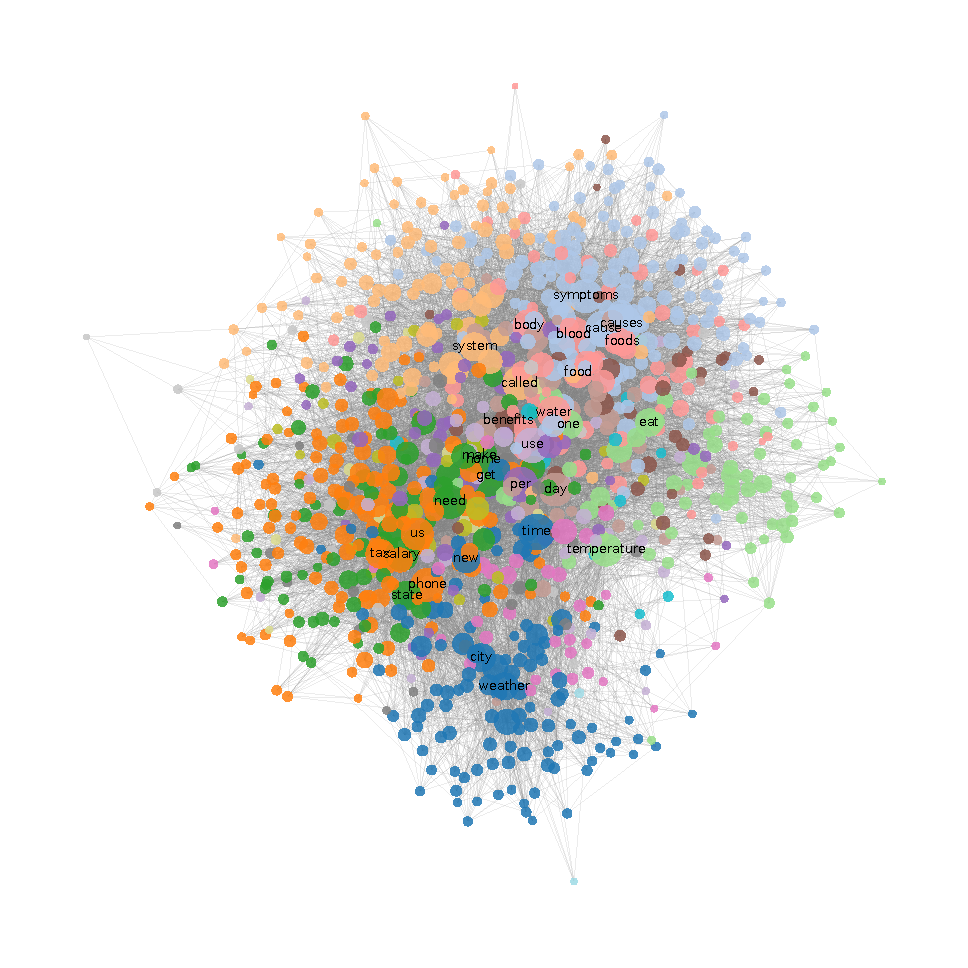
\includegraphics[width=0.8\textwidth]{leiden/graph_clusters.pdf}
	\caption{Term co-occurrence graph: the 1000 highest-degree terms, colour = Leiden cluster, vertex size = weighted degree}
	\label{fig:graph}
\end{figure}

\begin{figure}[H]
	\centering
	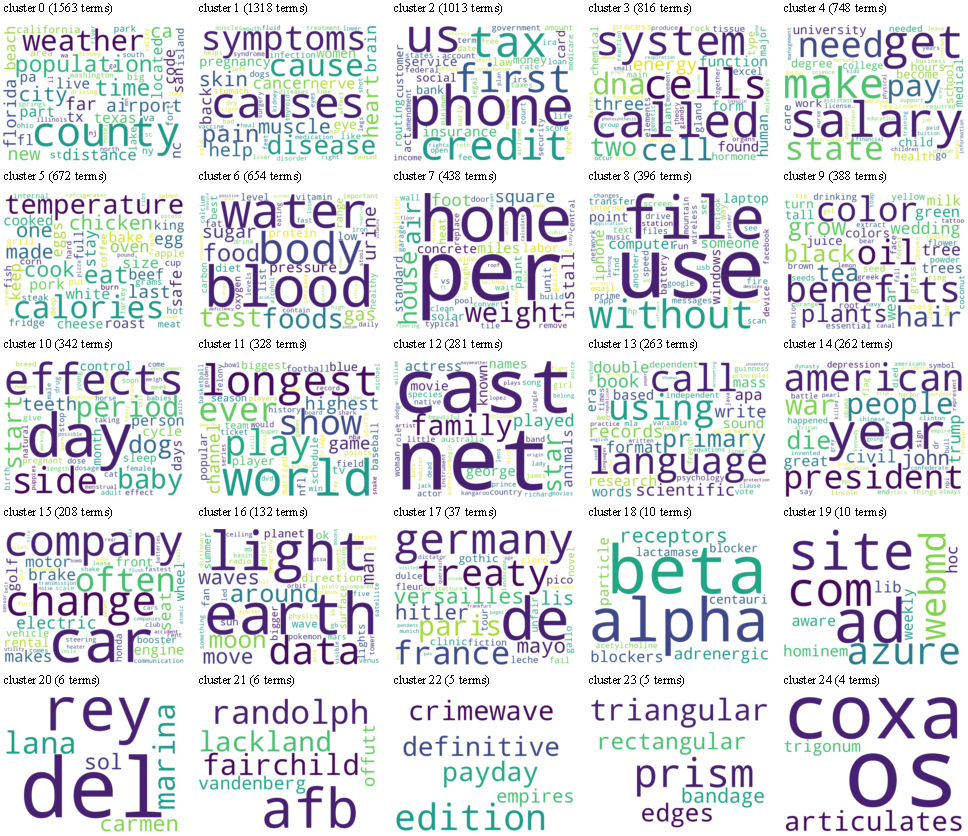
\includegraphics[width=\textwidth]{leiden/cluster_wordclouds.pdf}
	\caption{Word clouds of the 25 largest Leiden clusters (word size proportional to the sum of its edge weights)}
	\label{fig:wordclouds}
\end{figure}

\begin{figure}[H]
	\centering
	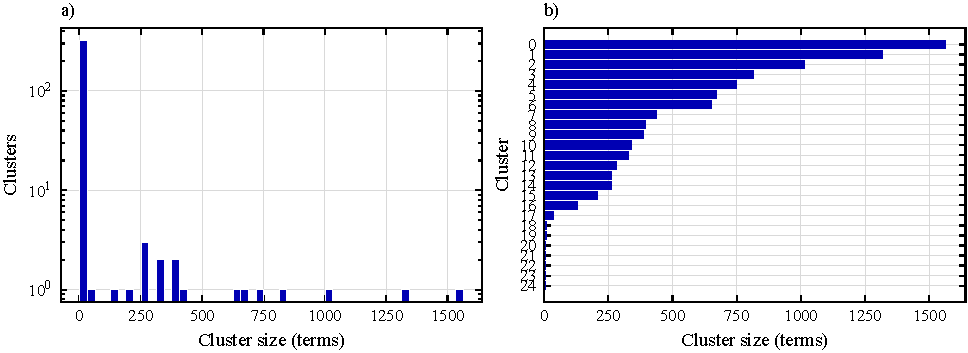
\includegraphics[width=\textwidth]{leiden/cluster_sizes.pdf}
	\caption{Leiden cluster sizes: log-scale histogram (a) and the 25 largest clusters (b)}
	\label{fig:cluster-sizes}
\end{figure}

\begin{figure}[H]
	\centering
	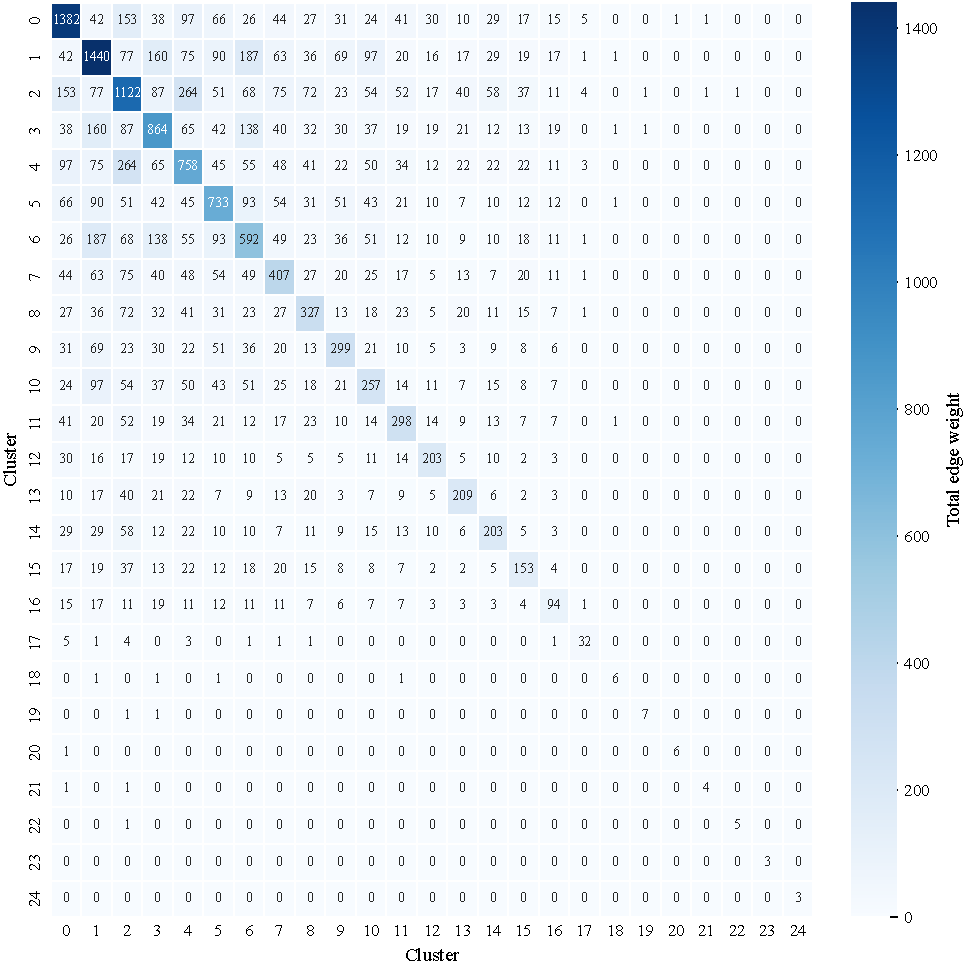
\includegraphics[width=0.85\textwidth]{leiden/cluster_heatmap.pdf}
	\caption{Total edge weight within and between the 25 largest Leiden clusters}
	\label{fig:heatmap}
\end{figure}

\subsection{Fighting the Degenerate Cluster}

\todo{Text: by Eq.~\eqref{eq:lower-bound} a cluster of frequent terms gathers most of the corpus (Leiden \strategy{aff}: largest shard \affLargest\,\%); attempts without a budget~--- tightening the algorithm's own parameter (Figure~\ref{fig:sweeps}): the largest shard shrinks but never reaches the budget while duplication grows and overlap falls together with volume; changing graph thresholds, edge weights and the vote rule (Figure~\ref{fig:variants-largest}): none of the 19~variants under any algorithm brings the shard within the budget; other algorithms (figure columns, Table~\ref{tab:methods}) give smaller clusters, still above the budget. Conclusion: an explicit volume budget is needed. Materials: Figure~\ref{fig:sweeps}; Figure~\ref{fig:variants-largest}.}

\begin{figure}[H]
	\centering
	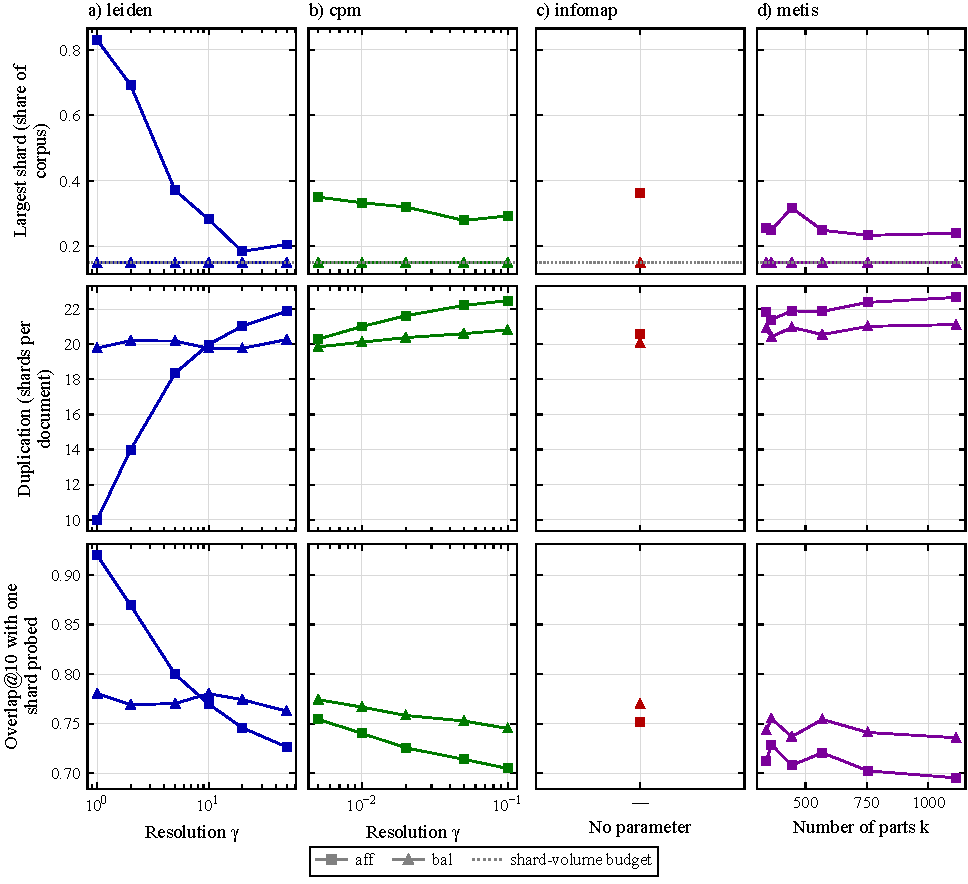
\includegraphics[width=\textwidth]{overview_parameter_sweeps.pdf}
	\caption{Largest shard, duplication and overlap@10 when probing one shard against the clustering algorithm's own parameter for \strategy{aff} and \strategy{bal}: Leiden (a), CPM (b), Infomap (c; no parameter of its own, the main configuration is shown), METIS (d); the dotted line is the shard-volume budget; held-out sample}
	\label{fig:sweeps}
\end{figure}

\begin{figure}[H]
	\centering
	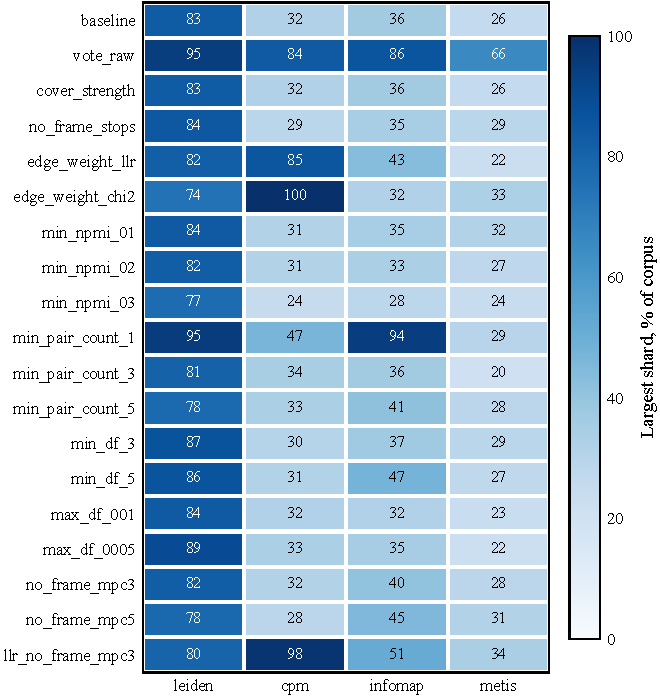
\includegraphics[width=0.75\textwidth]{overview_variants_largest_shard.pdf}
	\caption{Share of the corpus in the largest shard of \strategy{aff} by configuration variant (rows) and clustering algorithm (columns), \%; the volume budget is 15\,\%}
	\label{fig:variants-largest}
\end{figure}

\subsection{Comparison of the Strategies}

\todo{Text: the three strategy families under Leiden (Table~\ref{tab:strategies}); the overlap of the unbudgeted families is bought with probed volume and a giant shard (Figure~\ref{fig:quality-cost}); the same under the other algorithms (Table~\ref{tab:methods}); the duplication--cover trade-off (Figure~\ref{fig:tradeoff}); the only balanced strategy is \strategy{bal}, hence the detailed comparison with the hash partition of the same shard count. Materials: Table~\ref{tab:strategies}; Table~\ref{tab:methods}; Figure~\ref{fig:quality-cost}; Figure~\ref{fig:tradeoff}; Table~\ref{tab:budgets} (optional).}

\begin{table}[H]
	\caption{Sharding strategies on the held-out sample (Leiden): shards, duplication, share of the corpus in the largest shard, mean cover length, share of single-shard queries, overlap@10 and probed volume under a budget of $b$ shards}
	\label{tab:strategies}
	\centering
	\small
	\resizebox{\textwidth}{!}{% АВТОГЕНЕРАЦИЯ / AUTOGENERATED: build_tables.py <- metrics/*.csv
\begin{tabular}{lrrrrrrrrrr}
\toprule
\textbf{Strategy} & \textbf{Shards} & \textbf{Dup.} & \textbf{Largest, \%} & \textbf{Fanout} & \textbf{One shard, \%} & \multicolumn{2}{c}{\textbf{Overlap@10}} & \multicolumn{3}{c}{\textbf{Probed volume, \%}} \\
 &  &  &  &  &  & @1 & @2 & @1 & @2 & full \\
\midrule
\texttt{hash\_base} & 680 & 25.7 & 15.7 & 3.23 & 6.6 & 0.651 & 0.954 & 3.9 & 8.0 & 15.2 \\
\texttt{base} & 680 & 16.6 & 79.4 & 2.61 & 13.8 & 0.796 & 0.982 & 35.0 & 67.4 & 94.1 \\
\texttt{base\_r2} & 680 & 19.3 & 95.9 & 2.31 & 19.6 & 0.839 & 0.989 & 52.1 & 89.2 & 110.3 \\
\texttt{base\_r3} & 680 & 21.1 & 98.4 & 2.18 & 23.2 & 0.852 & 0.990 & 58.4 & 92.6 & 108.7 \\
\texttt{hash\_aff} & 400 & 25.3 & 19.8 & 3.22 & 6.6 & 0.660 & 0.957 & 6.5 & 12.9 & 23.2 \\
\texttt{aff} & 400 & 10.0 & 83.1 & 2.31 & 22.7 & 0.920 & 0.997 & 59.5 & 104.5 & 136.5 \\
\texttt{aff\_r2} & 400 & 12.2 & 96.4 & 1.98 & 31.3 & 0.952 & 0.999 & 75.7 & 126.8 & 149.4 \\
\texttt{aff\_r3} & 400 & 13.8 & 98.6 & 1.85 & 36.5 & 0.962 & 0.999 & 82.4 & 132.6 & 150.1 \\
\texttt{hash\_bal} & 132 & 23.6 & 31.6 & 3.20 & 6.7 & 0.697 & 0.966 & 17.9 & 35.3 & 60.1 \\
\texttt{bal} & 132 & 19.8 & 15.0 & 2.90 & 9.4 & 0.780 & 0.979 & 15.0 & 28.5 & 43.4 \\
\bottomrule
\end{tabular}
}
\end{table}

\begin{table}[H]
	\caption{Share of the corpus in the largest shard, overlap@10 and probed volume when probing one shard by strategy and clustering algorithm (held-out sample)}
	\label{tab:methods}
	\centering
	\small
	\resizebox{\textwidth}{!}{% АВТОГЕНЕРАЦИЯ / AUTOGENERATED: build_tables.py <- metrics/*.csv
\begin{tabular}{lrrrrrrrrrrrr}
\toprule
\textbf{Strategy} & \multicolumn{4}{c}{\textbf{Largest shard, \%}} & \multicolumn{4}{c}{\textbf{Overlap@10 ($b=1$)}} & \multicolumn{4}{c}{\textbf{Probed volume ($b=1$), \%}} \\
 & Leiden & CPM & Infomap & METIS & Leiden & CPM & Infomap & METIS & Leiden & CPM & Infomap & METIS \\
\midrule
\texttt{hash\_base} & 15.7 & 12.0 & 11.9 & 15.3 & 0.651 & 0.640 & 0.642 & 0.652 & 3.9 & 0.7 & 1.2 & 3.9 \\
\texttt{base} & 79.4 & 19.3 & 27.8 & 18.6 & 0.796 & 0.680 & 0.697 & 0.660 & 35.0 & 1.5 & 3.3 & 3.9 \\
\texttt{base\_r2} & 95.9 & 47.7 & 60.1 & 24.2 & 0.839 & 0.721 & 0.743 & 0.700 & 52.1 & 6.6 & 11.4 & 6.7 \\
\texttt{base\_r3} & 98.4 & 57.6 & 67.6 & 35.4 & 0.852 & 0.741 & 0.762 & 0.726 & 58.4 & 9.5 & 15.5 & 9.4 \\
\texttt{hash\_aff} & 19.8 & 12.4 & 15.0 & 15.3 & 0.660 & 0.642 & 0.645 & 0.659 & 6.5 & 1.2 & 2.3 & 6.4 \\
\texttt{aff} & 83.1 & 32.0 & 36.3 & 25.5 & 0.920 & 0.726 & 0.752 & 0.713 & 59.5 & 3.3 & 6.6 & 6.8 \\
\texttt{aff\_r2} & 96.4 & 51.6 & 62.3 & 31.0 & 0.952 & 0.770 & 0.798 & 0.758 & 75.7 & 9.5 & 16.0 & 11.4 \\
\texttt{aff\_r3} & 98.6 & 60.6 & 70.4 & 36.0 & 0.962 & 0.790 & 0.818 & 0.787 & 82.4 & 12.9 & 20.9 & 15.4 \\
\texttt{hash\_bal} & 31.6 & 31.6 & 28.3 & 26.3 & 0.697 & 0.697 & 0.698 & 0.698 & 17.9 & 17.5 & 17.8 & 17.0 \\
\texttt{bal} & 15.0 & 15.0 & 15.0 & 15.0 & 0.780 & 0.758 & 0.770 & 0.743 & 15.0 & 14.9 & 14.9 & 14.9 \\
\bottomrule
\end{tabular}
}
\end{table}

\begin{figure}[H]
	\centering
	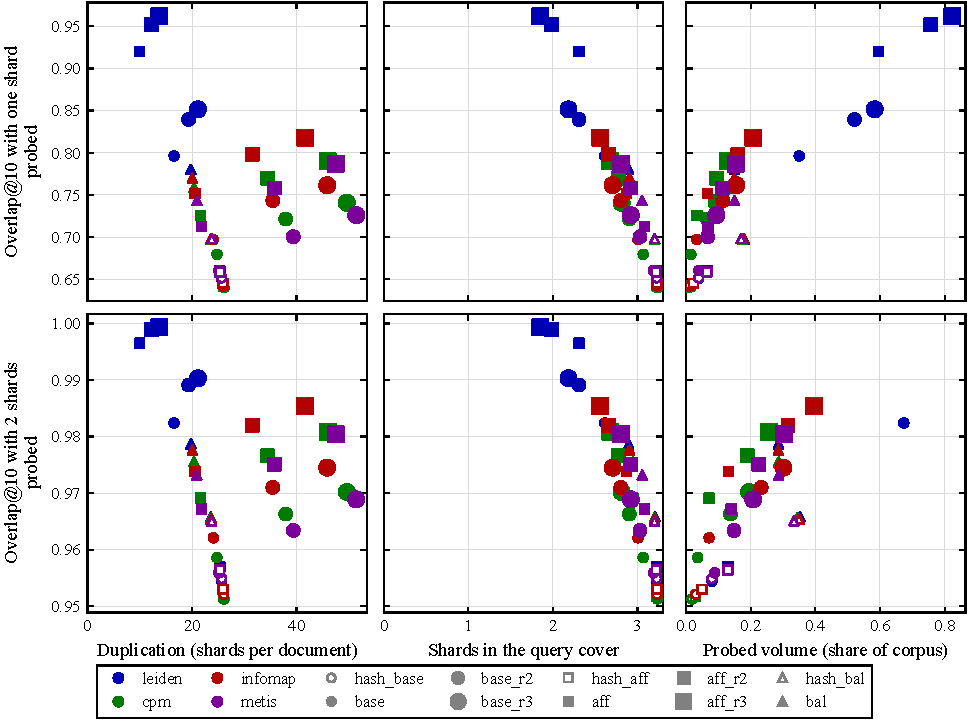
\includegraphics[width=\textwidth]{overview_quality_vs_cost.pdf}
	\caption{Overlap@10 when probing one (top row) and two (bottom row) shards against duplication, mean cover length and probed volume; all algorithms and strategies, held-out sample}
	\label{fig:quality-cost}
\end{figure}

\begin{figure}[H]
	\centering
	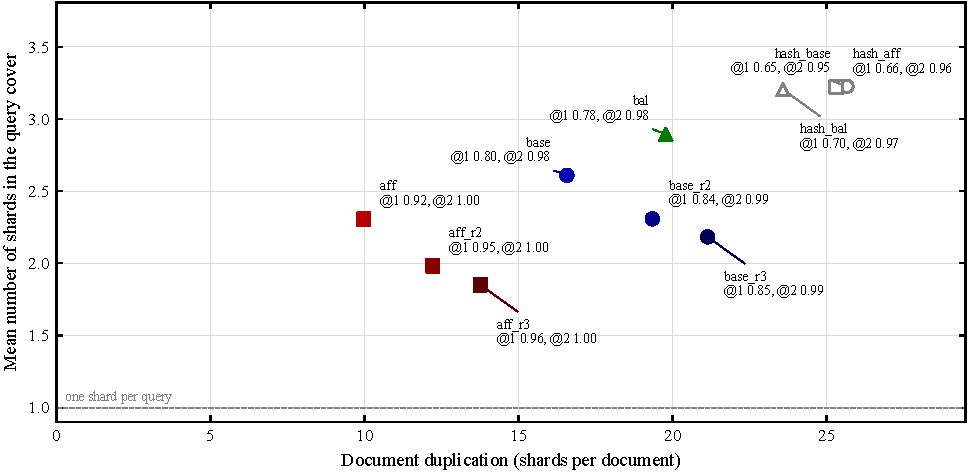
\includegraphics[width=\textwidth]{leiden/duplication_vs_fanout.pdf}
	\caption{Document duplication and mean cover length by strategy (Leiden, held-out sample); labels give overlap@10 when probing one and two shards}
	\label{fig:tradeoff}
\end{figure}

\begin{table}[H]
	\caption{Overlap@10 and probed volume under a budget of $b$ shards (Leiden, held-out sample)}
	\label{tab:budgets}
	\centering
	\small
	% АВТОГЕНЕРАЦИЯ / AUTOGENERATED: build_tables.py <- metrics/*.csv
\begin{tabular}{lrrrrrrrrrr}
\toprule
\textbf{Strategy} & \multicolumn{5}{c}{\textbf{Overlap@10}} & \multicolumn{5}{c}{\textbf{Probed volume, \% of corpus}} \\
 & $b=1$ & $b=2$ & $b=3$ & $b=5$ & full & $b=1$ & $b=2$ & $b=3$ & $b=5$ & full \\
\midrule
\texttt{hash\_base} & 0.651 & 0.954 & 0.996 & 1.000 & 1.000 & 4 & 8 & 12 & 15 & 15 \\
\texttt{base} & 0.796 & 0.982 & 0.999 & 1.000 & 1.000 & 35 & 67 & 86 & 93 & 94 \\
\texttt{base\_r2} & 0.839 & 0.989 & 1.000 & 1.000 & 1.000 & 52 & 89 & 106 & 110 & 110 \\
\texttt{base\_r3} & 0.852 & 0.990 & 1.000 & 1.000 & 1.000 & 58 & 93 & 105 & 108 & 109 \\
\texttt{hash\_aff} & 0.660 & 0.957 & 0.996 & 1.000 & 1.000 & 6 & 13 & 18 & 23 & 23 \\
\texttt{aff} & 0.920 & 0.997 & 1.000 & 1.000 & 1.000 & 59 & 105 & 127 & 136 & 137 \\
\texttt{aff\_r2} & 0.952 & 0.999 & 1.000 & 1.000 & 1.000 & 76 & 127 & 145 & 149 & 149 \\
\texttt{aff\_r3} & 0.962 & 0.999 & 1.000 & 1.000 & 1.000 & 82 & 133 & 148 & 150 & 150 \\
\texttt{hash\_bal} & 0.697 & 0.966 & 0.997 & 1.000 & 1.000 & 18 & 35 & 49 & 59 & 60 \\
\texttt{bal} & 0.780 & 0.979 & 0.998 & 1.000 & 1.000 & 15 & 29 & 38 & 43 & 43 \\
\bottomrule
\end{tabular}

\end{table}

\subsection{Balanced Strategy against Hash}

\todo{Text: at an equal number of shards \strategy{bal} beats \strategy{hash\_bal} on overlap and is cheaper in volume at every budget and under every algorithm (Figure~\ref{fig:budget-curves}, Table~\ref{tab:gains}); transfer across samples and frequent queries (Figure~\ref{fig:by-sample}, Table~\ref{tab:samples}); the distribution of the cover length (Figure~\ref{fig:fanout-ecdf}); the gain grows with connectivity and query length (Table~\ref{tab:slices}, Figure~\ref{fig:slices}). Materials: Figure~\ref{fig:budget-curves}; Table~\ref{tab:gains}; Figure~\ref{fig:by-sample}; Table~\ref{tab:samples}; Figure~\ref{fig:fanout-ecdf} (optional); Table~\ref{tab:slices}; Figure~\ref{fig:slices}.}

\begin{figure}[H]
	\centering
	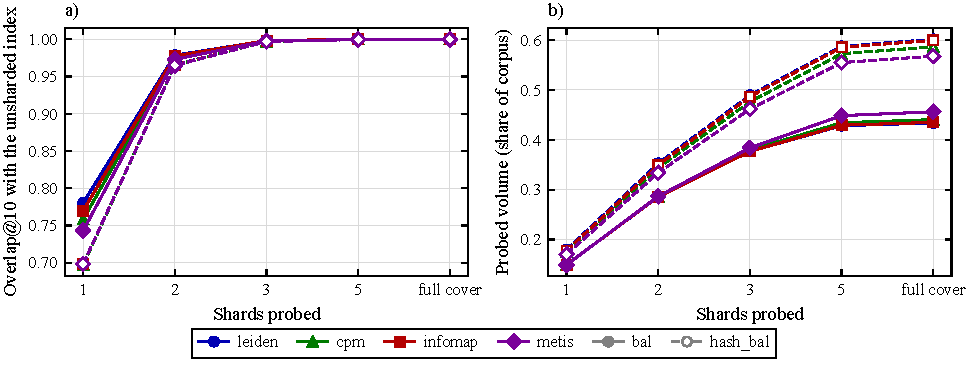
\includegraphics[width=\textwidth]{overview_budget_curves.pdf}
	\caption{\strategy{bal} against \strategy{hash\_bal} at an equal number of shards: overlap@10 (a) and probed volume (b) against the number of probed shards for the four clustering algorithms (held-out sample)}
	\label{fig:budget-curves}
\end{figure}

\begin{table}[H]
	\caption{Paired differences of \strategy{bal} against \strategy{hash\_bal} by clustering algorithm on the held-out and OOD samples: mean and 95\,\% confidence interval; volume in corpus fractions}
	\label{tab:gains}
	\centering
	\small
	\resizebox{\textwidth}{!}{% АВТОГЕНЕРАЦИЯ / AUTOGENERATED: build_tables.py <- metrics/*.csv
\begin{tabular}{llccccc}
\toprule
\textbf{Sample} & \textbf{Algorithm} & \textbf{$\Delta$ overlap@10 ($b=1$)} & \textbf{$\Delta$ overlap@10 ($b=2$)} & \textbf{$\Delta$ fanout} & \textbf{$\Delta$ one shard} & \textbf{$\Delta$ volume@1} \\
\midrule
holdout & Leiden & +0.083 [0.077,\,0.089] & +0.013 [0.011,\,0.015] & $-$0.31 [$-$0.33,\,$-$0.29] & +0.027 [0.023,\,0.031] & $-$0.030 [$-$0.031,\,$-$0.029] \\
holdout & CPM & +0.061 [0.056,\,0.067] & +0.010 [0.008,\,0.012] & $-$0.26 [$-$0.27,\,$-$0.24] & +0.020 [0.016,\,0.024] & $-$0.025 [$-$0.026,\,$-$0.024] \\
holdout & Infomap & +0.072 [0.066,\,0.078] & +0.012 [0.010,\,0.015] & $-$0.30 [$-$0.31,\,$-$0.28] & +0.023 [0.019,\,0.027] & $-$0.028 [$-$0.029,\,$-$0.027] \\
holdout & METIS & +0.045 [0.040,\,0.050] & +0.008 [0.006,\,0.010] & $-$0.15 [$-$0.16,\,$-$0.14] & +0.014 [0.011,\,0.017] & $-$0.021 [$-$0.022,\,$-$0.020] \\
OOD & Leiden & +0.109 [0.104,\,0.114] & +0.038 [0.034,\,0.041] & $-$0.37 [$-$0.38,\,$-$0.35] & +0.003 [0.002,\,0.004] & $-$0.030 [$-$0.031,\,$-$0.029] \\
OOD & CPM & +0.096 [0.090,\,0.101] & +0.034 [0.031,\,0.037] & $-$0.36 [$-$0.37,\,$-$0.34] & +0.002 [0.001,\,0.003] & $-$0.026 [$-$0.027,\,$-$0.025] \\
OOD & Infomap & +0.106 [0.101,\,0.111] & +0.038 [0.034,\,0.041] & $-$0.39 [$-$0.40,\,$-$0.37] & +0.003 [0.002,\,0.004] & $-$0.028 [$-$0.029,\,$-$0.028] \\
OOD & METIS & +0.060 [0.055,\,0.065] & +0.021 [0.018,\,0.024] & $-$0.19 [$-$0.20,\,$-$0.18] & +0.001 [0.000,\,0.001] & $-$0.022 [$-$0.022,\,$-$0.021] \\
\bottomrule
\end{tabular}
}
\end{table}

\begin{figure}[H]
	\centering
	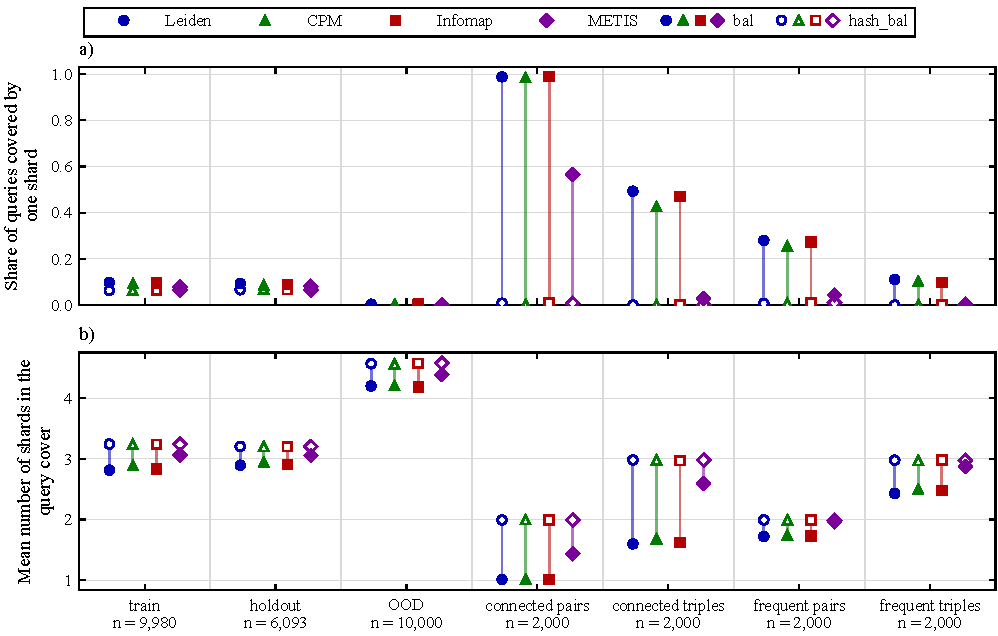
\includegraphics[width=\textwidth]{overview_by_sample.pdf}
	\caption{Share of queries covered by a single shard (a) and mean cover length (b) across the seven samples: \strategy{bal} against \strategy{hash\_bal} for the four clustering algorithms; bars are 95\,\% confidence intervals}
	\label{fig:by-sample}
\end{figure}

\begin{table}[H]
	\caption{Seven query samples (Leiden): overlap@10 when probing one shard, share of single-shard queries and mean cover length for \strategy{bal} and \strategy{hash\_bal}}
	\label{tab:samples}
	\centering
	\small
	\resizebox{\textwidth}{!}{% АВТОГЕНЕРАЦИЯ / AUTOGENERATED: build_tables.py <- metrics/*.csv
\begin{tabular}{lrrrrrrr}
\toprule
\textbf{Sample} & \textbf{$n$} & \multicolumn{3}{c}{\textbf{\texttt{bal}}} & \multicolumn{3}{c}{\textbf{\texttt{hash\_bal}}} \\
 & & overlap@10 & one shard, \% & fanout & overlap@10 & one shard, \% & fanout \\
\midrule
train & 9,980 & 0.797 & 9.7 & 2.81 & 0.696 & 6.3 & 3.24 \\
holdout & 6,093 & 0.780 & 9.4 & 2.90 & 0.697 & 6.7 & 3.20 \\
OOD & 10,000 & 0.664 & 0.4 & 4.20 & 0.555 & 0.1 & 4.57 \\
connected pairs & 2,000 & 1.000 & 98.8 & 1.01 & 0.873 & 0.8 & 1.99 \\
connected triples & 2,000 & 0.992 & 49.3 & 1.60 & 0.864 & 0.0 & 2.98 \\
frequent pairs & 2,000 & 1.000 & 28.0 & 1.72 & 1.000 & 0.7 & 1.99 \\
frequent triples & 2,000 & 0.986 & 11.1 & 2.43 & 0.973 & 0.0 & 2.98 \\
\bottomrule
\end{tabular}
}
\end{table}

\begin{figure}[H]
	\centering
	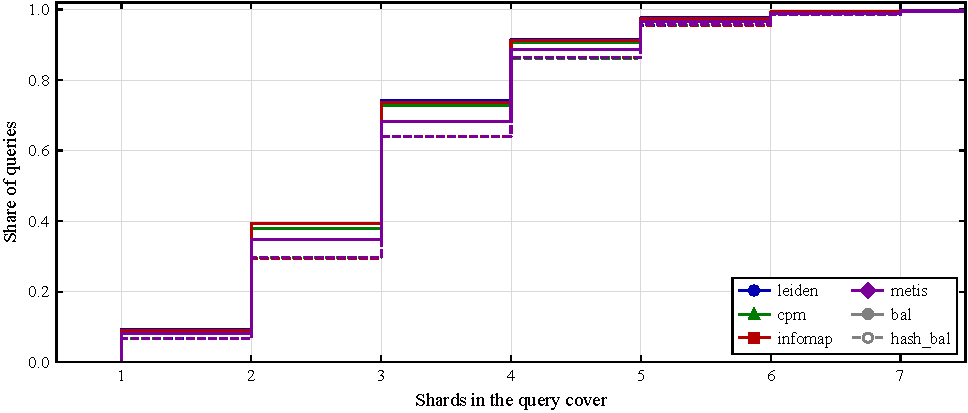
\includegraphics[width=\textwidth]{overview_fanout_ecdf.pdf}
	\caption{Empirical distribution of the number of shards in the query cover: \strategy{bal} (solid) against \strategy{hash\_bal} (dashed) for the four clustering algorithms (held-out sample)}
	\label{fig:fanout-ecdf}
\end{figure}

\begin{table}[H]
	\caption{Slices of the held-out sample by term connectivity (quartiles of mean NPMI, out-of-graph queries, single graph term) and by query length (Leiden)}
	\label{tab:slices}
	\centering
	\small
	\resizebox{\textwidth}{!}{% АВТОГЕНЕРАЦИЯ / AUTOGENERATED: build_tables.py <- metrics/*.csv
\begin{tabular}{lrrrrrrr}
\toprule
\textbf{Slice} & \textbf{$n$} & \multicolumn{3}{c}{\textbf{\texttt{bal}}} & \multicolumn{3}{c}{\textbf{\texttt{hash\_bal}}} \\
 & & fanout & overlap@10 ($b=1$) & overlap@10 ($b=2$) & fanout & overlap@10 ($b=1$) & overlap@10 ($b=2$) \\
\midrule
Q1 & 645 & 2.66 & 0.837 & 0.989 & 2.69 & 0.827 & 0.988 \\
Q2 & 264 & 3.88 & 0.772 & 0.969 & 4.14 & 0.711 & 0.961 \\
Q3 & 454 & 3.26 & 0.865 & 0.992 & 3.73 & 0.758 & 0.978 \\
Q4 & 454 & 2.53 & 0.950 & 1.000 & 3.36 & 0.847 & 0.992 \\
out of graph & 4,221 & 2.89 & 0.742 & 0.974 & 3.18 & 0.650 & 0.958 \\
single term & 55 & 1.00 & 1.000 & 1.000 & 1.00 & 1.000 & 1.000 \\
terms: 1 & 375 & 1.00 & 1.000 & 1.000 & 1.00 & 1.000 & 1.000 \\
terms: 2 & 1,346 & 1.90 & 0.797 & 1.000 & 1.98 & 0.759 & 1.000 \\
terms: 3 & 2,100 & 2.71 & 0.747 & 0.994 & 2.97 & 0.665 & 0.990 \\
terms: 4 & 1,398 & 3.50 & 0.761 & 0.960 & 3.95 & 0.652 & 0.939 \\
terms: 5+ & 874 & 4.72 & 0.773 & 0.931 & 5.41 & 0.622 & 0.883 \\
\bottomrule
\end{tabular}
}
\end{table}

\begin{figure}[H]
	\centering
	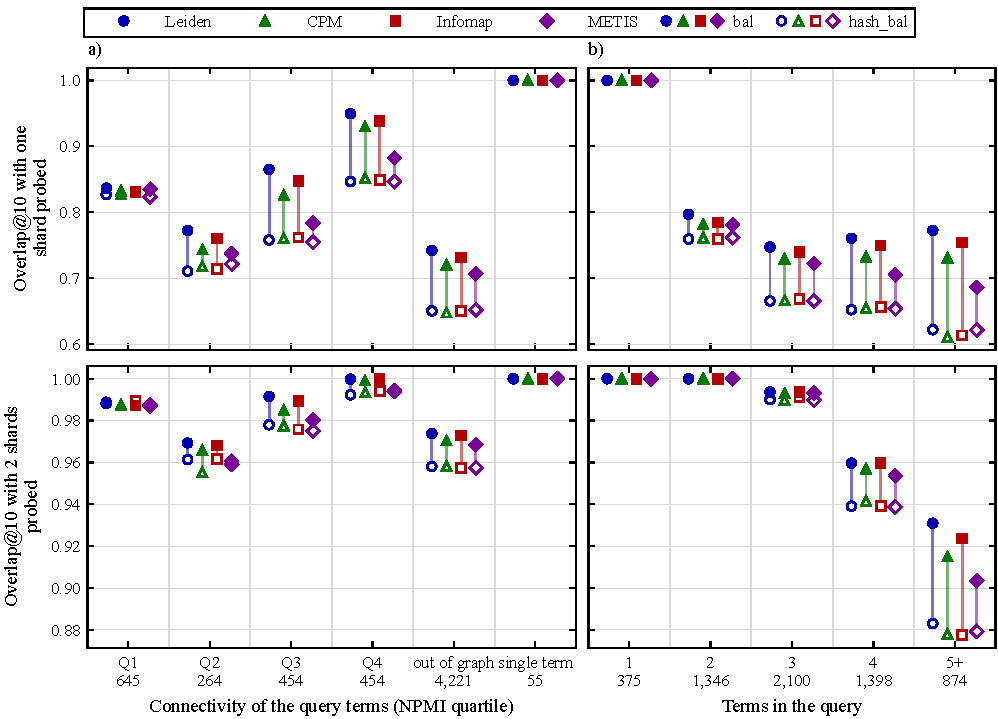
\includegraphics[width=\textwidth]{overview_slices.pdf}
	\caption{Overlap@10 when probing one (top row) and two (bottom row) shards by slices of the held-out sample: quartiles of term connectivity (a) and query length (b); \strategy{bal} against \strategy{hash\_bal} for the four algorithms}
	\label{fig:slices}
\end{figure}

\subsection{Correctness and Reproducibility}
\label{sec:verification}

\todo{Text: assignment recomputed from texts, cover completeness for all queries, comparison with real Whoosh shard indexes; software, seeds, DVC, repository. Materials: Table~\ref{tab:verification}.}

\begin{table}[H]
	\caption{Correctness check: computed results against real shard indexes}
	\label{tab:verification}
	\centering
	\small
	\resizebox{\textwidth}{!}{% АВТОГЕНЕРАЦИЯ / AUTOGENERATED: build_tables.py <- metrics/*.csv
\begin{tabular}{lrrrrcr}
\toprule
\textbf{Algorithm} & \textbf{Queries checked} & \textbf{Incomplete covers} & \textbf{Shard indexes built} & \textbf{Scores compared} & \textbf{Max $|\Delta|$ score} & \textbf{Result mismatches} \\
\midrule
Leiden & 34,073 & 0 & 86 & 434,954 & $3.6\cdot10^{-15}$ & 0 \\
CPM & 34,073 & 0 & 115 & 379,329 & $3.6\cdot10^{-15}$ & 0 \\
Infomap & 34,073 & 0 & 109 & 388,839 & $3.6\cdot10^{-15}$ & 0 \\
METIS & 34,073 & 0 & 109 & 391,564 & $3.6\cdot10^{-15}$ & 0 \\
\bottomrule
\end{tabular}
}
\end{table}

\subsection{Hyperparameter Selection}

\todo{Text: this is a check of the main configuration (Table~\ref{tab:configuration}), not its selection: the variants were measured after the main results on the same held-out sample and the configuration was not changed (the best variant gives Leiden +1.1~p.p. but CPM $-$2.4). Robustness of \strategy{bal} to the seed and the log size (Table~\ref{tab:sensitivity}); the algorithm's own parameter~--- the budget absorbs the resolution (Table~\ref{tab:parameters}); one setting changed at a time (Table~\ref{tab:variants}, Figure~\ref{fig:variants-overlap}): the effects on \strategy{bal} are small, the main configuration is close to the optimum. Materials: Table~\ref{tab:sensitivity}; Table~\ref{tab:parameters} (optional); Table~\ref{tab:variants}; Figure~\ref{fig:variants-overlap}.}

\begin{table}[H]
	\caption{Robustness of \strategy{bal} to the random seed (three seeds plus the main one) and to the number of training queries that build the graph}
	\label{tab:sensitivity}
	\centering
	\small
	\resizebox{\textwidth}{!}{% АВТОГЕНЕРАЦИЯ / AUTOGENERATED: build_tables.py <- metrics/*.csv
\begin{tabular}{lcccrrrr}
\toprule
\textbf{Algorithm} & \multicolumn{3}{c}{\textbf{Seeds (min--max)}} & \multicolumn{4}{c}{\textbf{Overlap@10 ($b=1$) by number of training queries}} \\
 & clusters & shards & overlap & 10,000 & 30,000 & 70,000 & 115,959 \\
\midrule
Leiden & 337--352 & 131--132 & 0.780--0.783 & 0.776 & 0.777 & 0.780 & 0.780 \\
CPM & 2,183--2,211 & 136--137 & 0.758--0.761 & 0.779 & 0.770 & 0.766 & 0.758 \\
Infomap & 1,114--1,121 & 134--135 & 0.768--0.770 & 0.771 & 0.774 & 0.773 & 0.770 \\
METIS & 335--335 & 140--140 & 0.741--0.743 & 0.777 & 0.764 & 0.762 & 0.743 \\
\bottomrule
\end{tabular}
}
\end{table}

\begin{table}[H]
	\caption{The clustering algorithm's own parameter and the \strategy{bal} strategy (held-out sample)}
	\label{tab:parameters}
	\centering
	\small
	\resizebox{\textwidth}{!}{% АВТОГЕНЕРАЦИЯ / AUTOGENERATED: build_tables.py <- metrics/*.csv
\begin{tabular}{lcrrrrrr}
\toprule
\textbf{Algorithm} & \textbf{Parameter} & \textbf{Value} & \textbf{Clusters} & \textbf{Shards} & \textbf{Fanout} & \textbf{Overlap@10 ($b=1$)} & \textbf{Overlap@10 ($b=2$)} \\
\midrule
Leiden & $\gamma$ & 1 & 340 & 132 & 2.90 & 0.780 & 0.979 \\
Leiden & $\gamma$ & 2 & 380 & 135 & 2.93 & 0.769 & 0.976 \\
Leiden & $\gamma$ & 5 & 439 & 135 & 2.94 & 0.770 & 0.977 \\
Leiden & $\gamma$ & 10 & 564 & 132 & 2.90 & 0.780 & 0.978 \\
Leiden & $\gamma$ & 20 & 747 & 132 & 2.90 & 0.774 & 0.978 \\
Leiden & $\gamma$ & 50 & 1,110 & 136 & 2.94 & 0.763 & 0.976 \\
CPM & $\gamma$ & 0.005 & 1,345 & 133 & 2.89 & 0.774 & 0.978 \\
CPM & $\gamma$ & 0.010 & 1,710 & 135 & 2.92 & 0.767 & 0.978 \\
CPM & $\gamma$ & 0.020 & 2,211 & 136 & 2.94 & 0.758 & 0.976 \\
CPM & $\gamma$ & 0.050 & 3,196 & 138 & 2.97 & 0.753 & 0.976 \\
CPM & $\gamma$ & 0.100 & 4,391 & 139 & 3.00 & 0.745 & 0.974 \\
METIS & $k$ & 341 & 335 & 140 & 3.05 & 0.743 & 0.973 \\
METIS & $k$ & 361 & 355 & 137 & 2.98 & 0.755 & 0.975 \\
METIS & $k$ & 444 & 432 & 140 & 3.08 & 0.737 & 0.973 \\
METIS & $k$ & 569 & 559 & 138 & 3.00 & 0.754 & 0.976 \\
METIS & $k$ & 754 & 718 & 141 & 3.05 & 0.741 & 0.974 \\
METIS & $k$ & 1113 & 1,029 & 141 & 3.06 & 0.736 & 0.975 \\
\bottomrule
\end{tabular}
}
\end{table}

\begin{table}[H]
	\caption{Configuration variants for \strategy{bal}: overlap@10 when probing one shard on the held-out sample and the change against the main configuration (percentage points) for the four clustering algorithms}
	\label{tab:variants}
	\centering
	\small
	\resizebox{\textwidth}{!}{% АВТОГЕНЕРАЦИЯ / AUTOGENERATED: build_tables.py <- metrics/*.csv
\begin{tabular}{lrrcccc}
\toprule
\textbf{Variant} & \textbf{Graph terms} & \textbf{Leiden clusters} & \textbf{Leiden} & \textbf{CPM} & \textbf{Infomap} & \textbf{METIS} \\
\midrule
\texttt{baseline} & 10,567 & 340 & 0.780 & 0.758 & 0.770 & 0.743 \\
\texttt{vote\_raw} & 10,567 & 340 & 0.776 ($-$0.4) & 0.758 (+0.0) & 0.766 ($-$0.4) & 0.734 ($-$0.9) \\
\texttt{cover\_strength} & 10,567 & 340 & 0.773 ($-$0.7) & 0.759 (+0.1) & 0.767 ($-$0.3) & 0.749 (+0.6) \\
\texttt{no\_frame\_stops} & 11,870 & 274 & 0.787 (+0.6) & 0.759 (+0.1) & 0.775 (+0.5) & 0.739 ($-$0.4) \\
\texttt{edge\_weight\_llr} & 10,567 & 356 & 0.788 (+0.7) & 0.746 ($-$1.3) & 0.780 (+1.0) & 0.756 (+1.3) \\
\texttt{edge\_weight\_chi2} & 10,567 & 552 & 0.777 ($-$0.4) & 0.714 ($-$4.4) & 0.767 ($-$0.3) & 0.749 (+0.6) \\
\texttt{min\_npmi\_01} & 10,566 & 347 & 0.782 (+0.2) & 0.759 (+0.1) & 0.767 ($-$0.3) & 0.740 ($-$0.3) \\
\texttt{min\_npmi\_02} & 10,538 & 336 & 0.783 (+0.2) & 0.758 (+0.0) & 0.769 ($-$0.1) & 0.742 ($-$0.1) \\
\texttt{min\_npmi\_03} & 10,201 & 364 & 0.782 (+0.1) & 0.762 (+0.4) & 0.766 ($-$0.4) & 0.747 (+0.4) \\
\texttt{min\_pair\_count\_1} & 21,785 & 55 & 0.777 ($-$0.3) & 0.753 ($-$0.6) & 0.750 ($-$2.0) & 0.771 (+2.8) \\
\texttt{min\_pair\_count\_3} & 5,621 & 254 & 0.783 (+0.3) & 0.773 (+1.5) & 0.780 (+1.0) & 0.753 (+1.0) \\
\texttt{min\_pair\_count\_5} & 2,699 & 196 & 0.783 (+0.3) & 0.783 (+2.4) & 0.780 (+1.0) & 0.774 (+3.1) \\
\texttt{min\_df\_3} & 9,504 & 219 & 0.779 ($-$0.1) & 0.764 (+0.6) & 0.770 (+0.0) & 0.742 ($-$0.2) \\
\texttt{min\_df\_5} & 7,743 & 88 & 0.778 ($-$0.2) & 0.765 (+0.6) & 0.772 (+0.2) & 0.760 (+1.7) \\
\texttt{max\_df\_001} & 9,897 & 351 & 0.779 ($-$0.1) & 0.760 (+0.2) & 0.766 ($-$0.4) & 0.755 (+1.2) \\
\texttt{max\_df\_0005} & 9,363 & 403 & 0.779 ($-$0.1) & 0.764 (+0.6) & 0.768 ($-$0.2) & 0.759 (+1.6) \\
\texttt{no\_frame\_mpc3} & 6,389 & 195 & 0.784 (+0.4) & 0.772 (+1.4) & 0.787 (+1.7) & 0.754 (+1.1) \\
\texttt{no\_frame\_mpc5} & 3,235 & 148 & 0.785 (+0.5) & 0.784 (+2.6) & 0.783 (+1.3) & 0.770 (+2.7) \\
\texttt{llr\_no\_frame\_mpc3} & 6,389 & 221 & 0.791 (+1.1) & 0.734 ($-$2.4) & 0.774 (+0.4) & 0.768 (+2.5) \\
\bottomrule
\end{tabular}
}
\end{table}

\begin{figure}[H]
	\centering
	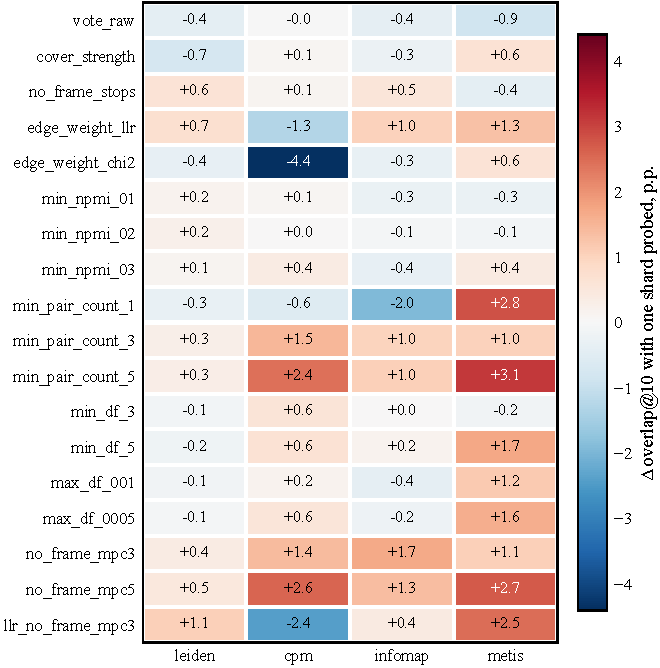
\includegraphics[width=0.75\textwidth]{overview_variants_overlap.pdf}
	\caption{Change of overlap@10 when probing one shard against the main configuration by configuration variant (rows) and clustering algorithm (columns), percentage points; \strategy{bal}, held-out sample}
	\label{fig:variants-overlap}
\end{figure}

\section{Limitations}

\todo{Text: the two regimes of the method; what the budget buys; comparison with selective search; tail latency; limitations (collection-wide BM25 statistics, one corpus and language, duplication of about 20, proxy costs instead of latency, synthetic samples favourable by construction, replicas under the budget not studied); future work. Materials: none.}

\section{Conclusion}

\todo{Text: one paragraph of problem statement, one of results with numbers (through the macros of \texttt{tables/numbers\_en.tex}), one of significance and future work. Materials: none.}

\bibliographystyle{unsrt}  % placeholder: numeric in citation order; the venue style replaces it
\bibliography{references}

\end{document}
